\documentclass{article}
% Package to manage page layout
\usepackage[margin=1.5cm, includefoot, footskip=30pt]{geometry}

\setlength\parindent{0pt}
\setlength{\parskip}{1em}

%%%%%%%PACKAGES HERE%%%%%%%
\usepackage{amsmath}
\usepackage{amssymb}
\usepackage{hyperref}
\usepackage{standalone}
\usepackage{subcaption}
\usepackage{tikz}
\usepackage{booktabs}
\usepackage{minted}
\usepackage{multicol}
\usetikzlibrary{er,positioning, calc}

\definecolor{background}{RGB}{5, 66, 81}
\usemintedstyle{tango}

\setcounter{secnumdepth}{4}
\setcounter{tocdepth}{4}

%%%%%%%%%%%%%%%%%%%%%%%%%%%%%%%PARAMETERS%%%%%%%%%%%%%%%%%%%%%%%%%%%%%%%%%%%%%%%
\newcommand{\totalarticles}{\input{assets/total_articles.txt}}
\newcommand{\uniquetitles}{\input{assets/unique_titles.txt}}
\newcommand{\numberofduplicates}{\input{assets/number_of_duplicates.txt}}
\newcommand{\manual}{\input{assets/prov_manual.txt}}
\newcommand{\authors}{\input{assets/authors.txt}}
\newcommand{\edges}{3174}
\newcommand{\auctionauthors}{\input{assets/authors_auction.txt}}
\newcommand{\auctionedges}{\input{assets/edges_auction.txt}}
\newcommand{\priceauthors}{\input{assets/authors_price.txt}}
\newcommand{\priceedges}{\input{assets/edges_price.txt}}
\newcommand{\prisonerscon}{\input{assets/prisoners_connected_components.txt}}
\newcommand{\prisonerscc}{\input{assets/prisoners_clustering.txt}}
\newcommand{\pricecon}{162}
\newcommand{\pricecc}{0.71}
\newcommand{\auctioncon}{\input{assets/auction_connected_components.txt}}
\newcommand{\auctioncc}{\input{assets/auction_clustering.txt}}
%%%%%%%%%%%%%%%%%%%%%%%%%%%%%%%%%%%%%%%%%%%%%%%%%%%%%%%%%%%%%%%%%%%%%%%%%%%%%%%%
%%%%%%%%%%%%%%%%%%%%%%%%%%%%%%%%%%%%%%%%%%%%%%%%%%%%%%%%%%%%%%%%%%%%%%%%%%%%%%%%
\title{A systematic literature review of the Prisoner's Dilemma and an analysis of the corresponding co author network.}
\author{Nikoleta E. Glynatsi}
\date{2016}

\begin{document}

\maketitle

\section{Introduction}\label{section:introduction}

The emergence of cooperation is a topic of continuing and public interest
for the social~\cite{capraro2014, gracia2012},
biological~\cite{Douglas2011}
and ecological sciences~\cite{Godfray1992,Krama2012,Milinski1987,Wilkinson1984}.
Cooperation is essential for evolution but according to Darwin's theory
it is not always easy to achieve. The game called the prisoner's
dilemma offers a theoretical framework for studying the emergence of
altruistic behaviour.

\subsection{The Prisoner's Dilemma}\label{section:prisoners_dilemma}

The prisoner's dilemma is a two player non-cooperative game~\cite{Flood1958} where
the decisions of the players are made simultaneously and independently. Both players
can choose between cooperation (\textbf{C}) or defection (\textbf{D}).

The fitness of each player is influenced by its own behaviour, and the behaviour
of the opponent. If both players choose to cooperate, both do better
than if both defect. However, a player has the temptation to deviate. If a
player was to defect while the other cooperates, the defector receives
more than if both had cooperated. The reward for mutual cooperation is \(R\),
for a mutual defection they receive \(P\), and for cooperation-defection,
the cooperator receives \(S\) where the defector receives \(T\). Thus, the game's
payoffs are given by,

\begin{equation} \label{eq:the_pd_payoffs}
    \begin{pmatrix}
    R & S \\ T & P
    \end{pmatrix}
\end{equation}

where \(T > R > P > S \) and \(2R > T + S\) are the conditions for a dilemma
to exist. Due to rational behaviour and the knowledge that an individual is tempted
to defect the game's equilibrium lies at a mutual defection and both players
receive a payoff of \(P\). Thus, the dominant strategy for the prisoner's dilemma
is \textbf{D}.

However, when the game is studied in a manner where prior outcomes matter, the
defecting choice is no longer necessarily the dominant choice. The repeated
form of the game is called the iterated prisoner's dilemma and now two players play
the game repeatedly. Interest was sparked on the iterated prisoner dilemma by
R. Axelrod and his book~\cite{Axelrod1984} ``The Evolution of Cooperation''.

In his book Axelrod reports on a series of computer tournaments he organised of
a finite turns games of the iterated prisoner's dilemma. Participants
had to choose between \textbf{C} and \textbf{D} again and again while having
memory of their previous encounters. Academics from several fields were invited
design computer strategies to compete in the tournament. The pioneer work of Axelrod
showed that greedy strategies did very poorly in the long run while more altruistic
strategies did better.

``The Evolution of Cooperation'' is considered a milestone in the field but it
is not the only one. On the contrary, the prisoner's dilemma has attracted much
attention ever since the game's origins. This is shown in Figure~\ref{fig:timeline},
which illustrates the number of  publications on the prisoner's dilemma per year
from the following sources:

\begin{multicols}{3}
    \begin{itemize}
        \item arXiv;
        \item PLOS;
        \item IEEE;
        \item Nature;
        \item Springer.
    \end{itemize}
\end{multicols}

The choice of sources is due to the fact that they have an open access Api, the
process of collecting the data (including criteria for inclusion of papers) and
the analysis will be described more comprehensively in Section~\ref{section:analysis}.

Each point of Figure~\ref{fig:timeline} marks the starting year of a time period.
Each of these time periods is reviewed and presented in~\ref{section:timeline},
as an extensive literature review. This paper is the review of this type, in
such detail since the origins to date.

Furthermore, in Section~\ref{section:analysis} a comprehensive data set of literature
regarding the prisoner's dilemma will be presented and analysed. This allow us to
review the amount of published academic articles as well as measure and explore
the collaborations within the field.

\begin{figure}[!htbp]
    \centering
    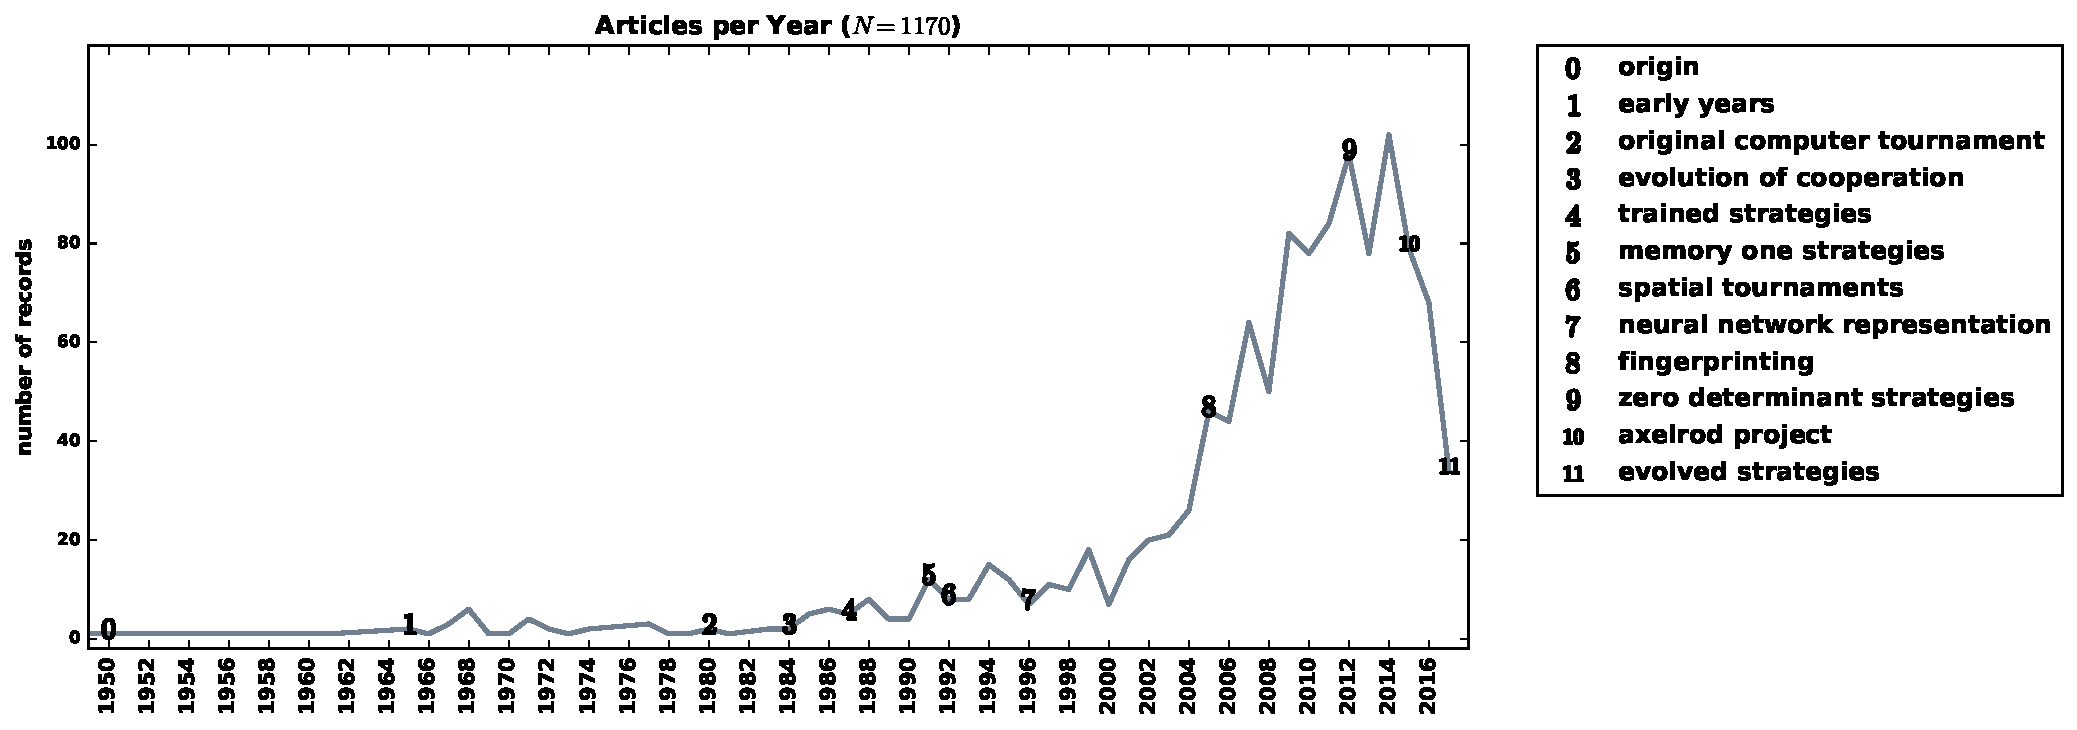
\includegraphics[width=\textwidth]{assets/images/timeline.pdf}
    \caption{\label{fig:timeline} A timeline of the prisoner's dilemma research.}
\end{figure}

\section{Timeline}\label{section:timeline}

\subsection{Origin and Primal research (1961-1972)}

The origin of the prisoner's dilemma goes back to the 1950s in early experiments
conducted in RAND~\cite{Flood1958} to test the applicability of games
described in~\cite{VonNeumann1944}. Although in~\cite{Flood1958} the two player
game was introduced the name behind the game was given later the same year.
According to~\cite{Tucker1983}, A. W. Tucker (the PhD supervisor of J. Nash),
in an attempt to delivery the game with a story during a talk used prisoners as
players and the game has been known as the prisoner's dilemma ever since~\cite{Tucker1983}.

The study of the prisoner's dilemma has attracted people from various fields
across the years. An early figure within the field is Prof A. Rapoport,
a mathematical psychologist, whose work focused on peacekeeping.
In his early work~\cite{rapoport1965} Rapoport conducted experiments using humans
to simulate a play of the prisoner's dilemma. Experimental groups were not been
used only by Rapoport but it was a common mean of studying the game
\cite{Evans1966, Gallo1968, Lutzker1961, Mack1971, Sensenig1972} and are still
being used today. %TODO reference a good article with human studies.

Those experiments explored the conditions under which altruist behaviour emerges
in human societies. Conditions such as, the gender~\cite{Evans1966,
Lutzker1961, Mack1971} of individuals, the representation of the game
\cite{Evans1966}, the distance between players~\cite{Sensenig1972}, the initial effects
\cite{Tedeschi1968} and whether the experimenter was biased~\cite{Gallo1968}.

Even though, several of these experiments were held and continuous research on
the topic was undergoing game theorists were still in disagreement about
the best way to play the game~\cite{rapoport1965}. Inspired by the work of
Rapoport and intrigued by the very same question the political scientist R.
Axelrod took upon himself to identify the dominant strategy of the prisoners dilemma.

The main difference of Axelrod's approach was that machines were going to be used
instead of humans. The issues with using humans, according to Axelrod
\cite{Axelrod2012}, was the fact that humans can act very randomly even though
the aim of the game is clear to them. Thus, Axelrod was the first researcher,
to the author's knowledge, to perform a computer tournament of the iterated
prisoner's dilemma. The work of Axelrod is considered one of the greatest
milestones within the field. The tournaments and their results are discussed in
the next sections.

\subsection{Axelrod's Tournaments (1981-1984)}\label{subsection:axelrods_tournament}

This section serves as a follow up from the earlier years of the topic and as an
introduction to the modern ways of studying the prisoner's dilemma. It is
dedicated to the computer tournaments of R. Axelrod from 1981 to 1984.

The first computer tournament was performed in 1980~\cite{Axelrod1980a}.
Several scientists were invited to submit their strategies, written in the
programming languages Fortran or Basic. There was a total number 13 submissions
made by the following researchers,

\begin{multicols}{2}
    \begin{enumerate}
        \item T Nicolaus Tideman and Paula Chieruzz;
        \item Rudy Nydegger;
        \item Bernard Grofman;
        \item Martin Shubik;
        \item Stein and Anatol Rapoport;
        \item James W Friedman;
        \item Morton Davis;
        \item Jim Graaskamp;
        \item Leslie Downing;
        \item Scott Feld;
        \item Johann Joss;
        \item Gordon Tullock;
        \item Name not given.
    \end{enumerate}
\end{multicols}

Each competed in a 200 turn match against all 13 opponents, itself and a player
that played randomly. This type of tournament is referred to as a round robin and
corresponds to a complete graph from a topological point of view. The tournament
was repeated \(5\) times to reduce variation in the results. Each participant knew
the exact length of the matches and had access to the full history of each match.
Furthermore, Axelrod performed an preliminary tournament and the results were known
to the participants. The payoff values used for~\ref{eq:the_pd_payoffs} where
\(R=3, P=1, T=5\) and \(S=0\). These values are commonly used in the literature
and unless specified will be the values used in the rest of the work described here.

The winner of the tournament was determined by the total average score and not by
the number of matches won. The strategy that was announced the winner was
submitted by Rapoport and was called \textbf{Tit For Tat}. Tit for Tat, is a
strategy that always cooperates on the first round and then mimics the opponent's
previous move.

Examples of Tit for Tat interacting for 8 turns with deterministic opponents are
given by Tables~\ref{table:tft_vs_c}, \ref{table:tft_vs_d}, \ref{table:tft_vs_a}.
The opponents are, \textbf{Cooperator} a strategy that always cooperates,
\textbf{Defector} an opponent that always defects and \textbf{Altenator} a
player who alternates between cooperating and defecting.

\begin{table}[!hbtp]
    \begin{center}
    \begin{tabular}{lcc}
        \toprule
        Turns & Tit for Tat & Cooperator\\
        \toprule
        1 & C & C \\
        2 & C & C \\
        3 & C & C \\
        4 & C & C \\
        5 & C & C \\
        6 & C & C \\
        7 & C & C \\
        8 & C & C \\
        \bottomrule
    \end{tabular}
    \caption{Tit for Tat example match of 8 turns against Cooperator}\label{table:tft_vs_c}
    \end{center}
\end{table}

\begin{table}[!hbtp]
    \begin{center}
    \begin{tabular}{lcc}
        \toprule
        Turns & Tit for Tat & Defector\\
        \toprule
        1 & C & D\\
        2 & D & D\\
        3 & D & D\\ 
        4 & D & D \\
        5 & D & D\\
        6 & D & D\\ 
        7 & D & D \\
        8 & D & D \\
        \bottomrule
    \end{tabular}
    \caption{Tit for Tat example match of 8 turns against Defector}\label{table:tft_vs_d}
\end{center}
\end{table}

\begin{table}[!hbtp]
    \begin{center}
    \begin{tabular}{lcc}
        \toprule
        Turns & Tit for Tat & Altenator\\
        \toprule
        1 & C & C \\ 
        2 & C & D \\ 
        3 & D & C \\ 
        4 & C & D \\
        5 & D & C \\ 
        6 & C & D \\ 
        7 & D & C \\ 
        8 & C & D \\
        \bottomrule
    \end{tabular}
    \caption{Tit for Tat example match of 8 turns against Altenator}\label{table:tft_vs_a}
\end{center}
\end{table}

The results of the first tournament were filled with surprises. Tit for Tat the
simplest strategy of all had won and had managed to defeat even entrants that
tried to improve on Tit for Tat after the preliminary tournament results.
Axelrod justified the success of the strategy saying that the strategy was
`nice' and `forgiving'.

The top eight ranked strategies were strategies that did no defect on the first
round, thus they were described as `nice' strategies. Compared to the rest of the
"nice" strategies, Tit for Tat had also another property. That property was
`forgiveness'. Tit for Tat punished it's opponent for a defection but just once
and then it would try to cooperate again. These two properties were described to
be the secret of success in a prisoner's dilemma tournament.

In order to further test the robustness of the results Axelrod performed a second
tournament~\cite{Axelrod1980b} later in 1980. This time a total of 63 participants
submitted strategies for the second tournament, their names were the following,

\begin{multicols}{3}
    \begin{enumerate}
        \item Gail Grisell;
        \item Harold Rabbie;
        \item James W Friedman;
        \item Abraham Getzler;
        \item Roger Hotz;
        \item George Lefevre;
        \item Nelson Weiderman;
        \item Tom Almy;
        \item Robert Adams;
        \item Herb Weiner;
        \item Otto Borufsen;
        \item R D Anderson;
        \item William Adams;
        \item Michael F McGurrin;
        \item Graham J Eatherley;
        \item Richard Hufford;
        \item George Hufford;
        \item Rob Cave;
        \item Rik Smoody;
        \item John Willaim Colbert;
        \item David A Smith;
        \item Henry Nussbacher;
        \item William H Robertson;
        \item Steve Newman;
        \item Stanley F Quayle;
        \item Rudy Nydegger;
        \item Glen Rowsam;
        \item Leslie Downing;
        \item Jim Graaskamp and Ken Katzen;
        \item Danny C Champion;
        \item Howard R Hollander;
        \item George Duisman;
        \item Brian Yamachi;
        \item Mark F Batell;
        \item Ray Mikkelson;
        \item Craig Feathers;
        \item Fransois Leyvraz;
        \item Johann Joss;
        \item Robert Pebly;
        \item James E Hall;
        \item Edward C White Jr;
        \item George Zimmerman;
        \item Edward Friedland;
        \item X	Edward Friedland;
        \item Paul D Harrington;
        \item David Gladstein;
        \item Scott Feld;
        \item Fred Mauk;
        \item Dennis Ambuehl and Kevin Hickey;
        \item Robyn M Dawes and Mark Batell;
        \item Martyn Jones;
        \item Robert A Leyland;
        \item Paul E Black;
        \item T Nicolaus Tideman and Paula Chieruzz;
        \item Robert B Falk and James M Langsted;
        \item Bernard Grofman;
        \item E E H Schurmann;
        \item Scott Appold;
        \item Gene Snodgrass;
        \item John Maynard Smith;
        \item Jonathan Pinkley;
        \item Anatol Rapoport.
    \end{enumerate}
\end{multicols}

All the participants knew the results of the previous tournament. The rules
were similar to those of the first tournament with only one exception;
the number of turns was not specified instead a fixed probability (refereed to as
`shadow of the future'~\cite{Axelrod1988}) of the game ending on the next move
was used. The fixed probability was chosen to be 0.0036 so that the expected
median length of a match would be 200 turns. The topology was of a round robin
and each pair of players was matched 5 times. The length of the matches was
determined once by drawing a random sample. Each of the five matches had a length
of 63, 77, 151 and 308.

The results of the tournament once again came as a surprise. Tit for Tat was
considered to be one of the simplest submissions in the second tournament and won
the second tournament as well.
Tit for Tat provided proof that reciprocity behaviour can allow cooperation
to emerge in the iterated prisoner's dilemma game. In~\cite{Axelrod1980a}
the main conclusions indicating strong performance was:

\begin{itemize}
    \item that it start of by cooperating
    \item it would forgive it's opponent after a defection
    \item after opponents identified that they were playing Tit for Tat choose
    to cooperate for the rest of the game.
\end{itemize}
%The strategies of the second tournament where bias due the first tournament. Discuss with V.

Another successful strategy from Axelrod's tournament that can been seen
in literature to date is \textbf{Grudger}, originally submitted by James W. Friedman.
Grudger is a strategy that will cooperate as long as the opponent does not defect.
The name Grudger was give to the strategy
in~\cite{Li2014}. Though the strategy goes by many names in the literature such as,
Spite~\cite{Beaufils1997}, Grim Trigger~\cite{Banks1990} and Grim~\cite{Van2015}.

As for the rest of the strategies, though a full explanation of all 13 submitted strategies
is given in~\cite{Axelrod1980a} the same does not hold for all 63 strategies of
the second tournament~\cite{Axelrod1980b}. The author mainly focuses on the high
ranked participants and several details for the rest strategies are left unknown.

The source code of the 63 strategies be found on Axelrod's personal
website~\cite{fortan_code}. The source code was written by Axelrod and several
other contributors. The strategies written in Basic were translated to
Fortran before the tournament. The source code includes the code only for the
strategies and not for creating and performing the tournament.Figure~\ref{fig:tit_for_tat_fortran}
serves as an example of the source code giving the code for the winning
strategy Tit for Tat. Unfortunately, the source code of the first 13 strategies
is not available, as stated in Axelrod's personal website~\cite{fortan_code}.

\begin{figure}[!hbtp]
    \centering
    \begin{minted}
        [
        autogobble=true,
        framesep=2mm,
        fontsize=\normalsize,
        ]
        {fortran}
    FUNCTION K92R(J,M,K,L,R, JA)
C BY ANATOL RAPOPORT
C TYPED BY AX 3/27/79 (SAME AS ROUND ONE TIT FOR TAT)
c replaced by actual code, Ax 7/27/93
c  T=0
c   K92R=ITFTR(J,M,K,L,T,R)
      k92r=0
      k92r = j
c test 7/30
c   write(6,77) j, k92r
c77   format(' test k92r. j,k92r: ', 2i3)
      RETURN
      END
    \end{minted}
    \caption{\label{fig:tit_for_tat_fortran} Source code for Tit for Tat in Fortran.
    Provided by~\cite{fortan_code}.}
\end{figure}

So far it has been discussed how the performance of the strategy has been tested
through tournaments against other strategies. A question remains: is the overall
success of a strategy based only on it's performance in a round robin tournament
or should it be checked through other ways as well?

Following his initial tournaments Axelrod performed an `ecological' tournament
in 1981~\cite{Axelrod1984}. Axelrod argued that some strategies are so unsuccessful
that there are very likely to be dropped in the future, while other more successful
strategies would continue in later interactions. Influenced by evolutionary biology
Axelrod introduced a way of capturing this behaviour, which included running a
series of tournaments where more successful strategies would occupy a larger part
of the environment and the less successful strategies would become less often.
This is known as an ecological tournament.

The simulation of the process, as described in~\cite{Axelrod1984}, is straightforward.
Consider matrix~\ref{eq:interaction_payoffs} which provides the expected payoff
when two individuals of different type interact. Starting with proportions of
each type in a given generation the proportions of these strategies in the next
generation is the only measure needed to be calculated. This is achieved by
calculating the weighted average of the scores of a given strategy with all
other players, where the weights are the numbers of the other strategies which
exist in the current generation. The numbers of a given strategy in the next
generation is then taken to be proportional to the product of its numbers in the
current generation and its score in the current generation.

\begin{equation} \label{eq:interaction_payoffs}
    \begin{pmatrix}
    (R=3, R=3) & (S=0, T=5) \\ (T=5, S=0) & (P=1, P=1)
    \end{pmatrix}
\end{equation}

Note the ecological tournament does not offer any evolutionary perspective.
There is no possibility of a new strategy to be introduced, there is no mutation
probability to drive the evolution. The ecological is a framework that provides
the distributions of given types over time when interacting with the population.

The set of strategies from Axelrod's second tournament was used to perform the
ecological tournament. Several interesting insights were reported,

\begin{itemize}
    \item The lowest ranking 11 strategies had fallen to half their initial size
    by the 5 generation;
    \item The middle-ranking entries managed to hold their initial size;
    \item By the \(500^{th}\) generation the only strategies that were larger than their
    initial size have been the top 11 ranked strategies;
    \item These formed 96\% of the population at that time;
    \item The rule which ranked fifth in the tournament, submitted by William Adams,
    grew to three times its original size in the population and then began to sink
    after generation 100;
    \item The rule which ranked eighth, submitted by Paul D. Harrington, and was
    the only non nice rule in the top 15, grew to four times its original size but
    began to shrink after generation 150 to reach only a third of its original
    size by the \(1000^{th}\) generation.
\end{itemize}

Overall the strategies that did rank at the top of the second tournament have
also ranked top in the ecological tournament. On the same note, the strategy that
was ranked at the top was again Tit for Tat. By the 1000th generation it was 14.5\%
of the whole population, followed by the third place rule at 13.9\% and then the
second place rue at 13.1\%, Tit for Tat was growing at .05\% per generation which
was a faster rate than any other strategy. All these ar captured in
Figure~\ref{fig:ecological.tournament}.

The ability of strategies to be favoured under natural selection and their
ability to withstand invasion from other strategies soon became a measure
of performance; refereed to as the stability of a strategy.

\begin{figure}[!hbtp]
    \centering
    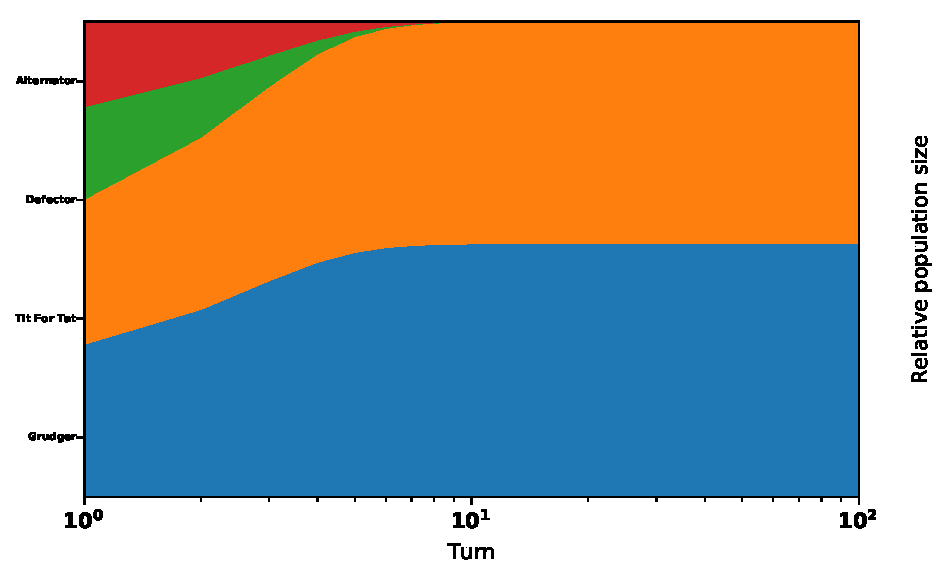
\includegraphics[width=.6\textwidth]{./assets/images/ecological.pdf}
    \caption{System evolving over time based on natural selection using
    \cite{axelrodproject}, strategies set from Axelord's second tournament.}
    \label{fig:ecological.tournament}
\end{figure}

A much more general approach was discussed in~\cite{axelrod1981}; the evolutionary
approach. Imagine a population made up of individuals where everyone follows the
same strategy, \(B\) and a single individual adopts a mutant strategy \(A\).
Strategy \(A\) is said to invade strategy \(B\) if,

\begin{equation}
V(A \mid B) > V(B \mid B)
\end{equation}
where \(V(B \mid B)\) is the expected payoff received by \(B\) against itself.

Since the strategy \(B\) is an population that interacts only with itself,
the concept of invasion is equivalent to a single mutant being able to outperform
the average population. This leads to the concept of the evolutionary approach.
Thus for a strategy to be \textbf{evolutionary stable} it must be able to
resists any invasion. There are several applications in biology for the interpretation
of this approach, for example the survival of the fitness in wildlife.

Due the large number of possible strategies in the prisoner's dilemma identifying
all the stable strategies was a difficulty task at the time. Axelrod focused
the work of~\cite{axelrod1981} in three questions,

\begin{enumerate}
    \item Under what conditions was Tit for Tat evolutionary stable?
    \item What were the necessary and sufficient conditions for any strategy to be
    evolutionary stable?
    \item Finally, in an environment where all followed a strategy of unconditional
    defection, can cooperation emerge?
\end{enumerate}

A series of theorems were presented which showed, that Tit for Tat is evolutionary
stable y if and only if it is invadable neither by Defector nor Alternator. This
is true only if the game is likely to last long enough for the retaliation
to counteract the temptation to defect, according to Axelrod. Secondly,
Defectors can withstand invasion by any strategy, as long as the players using
other strategies come one at a time. But if they come in clusters (even in rather small
clusters), the strategy could be invaded. As for the characteristics of stable
strategies, Axelrod provided a series of theorems.

\subsubsection{Response to the computer tournaments (1984-1993)}

The pioneering work of computer tournaments and the results on the reciprocal behaviour
of the prisoner's dilemma spread the knowledge of the game not only worldwide
but also across different scientific principles. The study of cooperation became
of critical interest once again. This section focuses on the immediate research
that was carried out after the initial computer tournaments.

Ecological studies that made use of Axelrod's results include the
works of~\cite{Godfray1992, Milinski1987, Wilkinson1984}, more specifically how
the successful strategy Tit for Tat can be applied in nature and wildlife.

In~\cite{Milinski1987} the behaviour of fish when confronting a potential predator
was studied. Conflicts can arise within pairs of fish in these circumstances.
Two experiments were held using a system of mirrors where sticklebacks would be
accompanied by  a cooperating companion or a defecting one. In both cases the hypothesis
that the fish would behave according to Tit for Tat and that cooperation would evolve
were supported. The works of~\cite{Godfray1992, Wilkinson1984} looked at
food sharing between vampire bats and explained behaviour based on famous at
that time tournament strategies.

Axelrod's tournaments assumed that each player has perfect information of the
opponent's actions. In real life situations this is not always the case.
Interactions often suffer from measures of uncertainty. In the original tournaments
there was no possibility of misunderstanding.

In 1985, P. Molander tested the robustness of Tit for Tat in an uncertain environment
by introducing noise~\cite{Molander1985}. Noise is a probability that that one's
move will be flipped. Molander findings stated that if two strategies playing Tit
for Tat meet in a noisy match the average payoff that a strategy will receive will
be the same as that of a Random player (with probability \(0.5\) of cooperating).

Further work on the performance of Tit for Tat in uncertain environments was
conducted, described in~\cite{Bendor1991, Godfray1992, Nowak1992}. These works
focused, similar to Molander's, focused on how the strategy suffers against itself
the most. In a noise environment, where a random defection can occur, the two
strategies would end up in an unwanted circle of defection-cooperation. In a non
noisy environment the strategies would have cooperated until the final interaction.

In~\cite{Bendor1991} a similar tournament to that of Axelrod's was performed
but this time noise was used. J. Bendor invited academics to submit strategies
to participate in the tournament. A total of thirteen strategies were used
including already existed strategies such as Tit for Tat and \textbf{Tit for Two
Tats}~\cite{Axelrod1988}. Tit for Two Tats is a variant of the classic strategy
that defects only when the opponent has defected twice in a row. The findings
of the tournaments suggested that a more forgiving strategy is needed in a noisy
environment. The winner of this tournament was a strategy called
\textbf{Nice and Forgiving}.

The work of~\cite{Nowak1992} aimed to also investigate stochastic effects.
Using an evolutionary setting of a heterogeneous population where noise is taken
into account, the space of reactive strategies was explored. Though a small fraction
of Tit for Tat players have been essential for the emergence of cooperation,
more generous strategies took over the population. This reactive strategy was
is known as \textbf{Generous Tit for Tat} and can be presented as \((0, \frac{2}{}3)\).

Reactive strategies are a subset of memory one strategies introduced in 1989~\cite{nowak1989}.
Reactive strategies are denoted by the probabilities to cooperate after an
opponent's \textbf{C} or \textbf{D} respectively. Thus, a reactive strategy only
considers the previous turn of the opponent. Memory one strategies, are a set of
strategies that consider the entire last turn of the game to decide on a next move.

Memory one strategies were also introduced by M. Nowak in 1990~\cite{Nowak1990}.
Depending on the simultaneous moves of two players the states of the game,
when only the previous round is considered, a state where both cooperated,
both defected or either of them defected. These states are represented as
\(CC, CD, DC, DD\). A memory one strategy can be written as the probability of
cooperating after each of these states. Thus as a vector of four probabilities
\(p\) where \( p = (p_1, p_2, p_3, p_4) \in\mathbb{R}_{[0,1]}^{4} \).
Reactive strategies are just a constrained version of memory one strategies where
\(p_1=p_3\) and \(p_2=p_1\).

The above formulation offered a new framework of studying strategies. Consider
that two memory one strategies are in a game of the prisoner's dilemma. Their
interaction can be written as the following markov chain,

\begin{equation}\label{eq:markov_matrix}
    M =
\begin{bmatrix}
    p_{1} q_{1} & p_{1} (- q_{1} + 1) & q_{1} (- p_{1} + 1) & (- p_{1} + 1) (- q_{1} + 1)
    \\
    p_{2} q_{3} & p_{2} (- q_{3} + 1) & q_{3} (- p_{2} + 1) & (- p_{2} + 1) (- q_{3} + 1)
    \\
    p_{3} q_{2} & p_{3} (- q_{2} + 1) & q_{2} (- p_{3} + 1) & (- p_{3} + 1) (- q_{2} + 1)
    \\
    p_{4} q_{4} & p_{4} (- q_{4} + 1) & q_{4} (- p_{4} + 1) & (- p_{4} + 1) (- q_{4} + 1)
    \\
\end{bmatrix}
\end{equation}

where the opponent is denoted as \(q=(q_1, q_2, q_3, q_4) \in\mathbb{R}_{[0,1]}^{4}\).
The expected state that two opponents will end up can be estimated by calculating
the steady states of the markov chain.

Nowak, as described, studied the reactive but also the memory one strategies
space and introduced several other strategies, among them the most popular was
\textbf{Pavlov}. Pavlov is a strategy with the tolerance of Generous Tit for Tat
but also the capability of resisting and invading an all-out cooperators population.
The strategy is based on the fundamental behavioural mechanism win-stay,
lose-shift. It starts off with a cooperation and then repeats it's previous move
only if it was awarder with a payoff of \(R\) or \(T\). Otherwise it shifts
it's last move.

A number of researchers searched for new strategies. Such strategies have been,
\textbf{Handshake}~\cite{Robson1989} and \textbf{Gradual}~\cite{Beaufils1997}.
Presented in 1989 and 1997 respectively.Handshake was developed using an
evolutionary tournament, where Gradual performance was tested in both a round-robin
tournament and ecological simulation.

Handshake is a strategy that starts with cooperation, defection. If the opponent
plays in a similar way then it will cooperate forever, otherwise it will defect
forever. Gradual starts off by cooperating, then after the first defection of the
other player, it defects one time and cooperates twice. After the second defection
of the opponent, it defects two times and cooperates twice. After the \(n^{th}\)
defection it reacts with \(n\) consecutive defections and then two cooperations.

Another measure of uncertainty is that of mis perception. Though noise will flip
a player's action it will be recorded correctly in the history. Mis perception is
the probability that the opponent's current move is flipped before being recorded
\cite{Hoffmann1998}.

\subsection{Evolutionary Dynamics (1987-1999)}

Determining the evolutionary stability of strategies for the iterated prisoner's
dilemma as we discussed is not an easy task. Methods can be use to deal with
the difficulty. In~~\cite{Boyd1987} the author restricted the possible strategies
that could be adopted to a relatively narrow set and resulted that no pure strategy
is evolutionary stable, including Tit for Tat. Arguing with the results presented
in~\cite{axelrod1981}. The list of strategies used included strategies such as
Defector and \textbf{Suspicious Tit for Tat}, a strategy that plays
Tit for Tat but starts by defecting.

The results were questioned by~\cite{May1987}, stating that much was still no fully
explored and more research had to be put into the results. Farrel and Ware in
1989~\cite{Farrell1989} extended the result to include finite mixture of pure
and mixtures of Tit For \(n\) Tats as well. On the same year the work of~\cite{Boyd1989}
looking again at a narrow set of strategies extended their results to
noisy environments.

Evolutionary dynamics have been highly useful in the research of the prisoner's
dilemma. In~\cite{Axelrod1987}, an evolutionary process, called the genetic
algorithm, was used to discover effective strategies. The author introduced
lookup tables as a mean of representing a strategy in a gene format. A lookup
table is a set of deterministic responses based on the opponents \(m\) last
moves; \cite{Axelrod1987} considered \(m=3\).

An extension to the natural selection was introduced in the 1992~\cite{Nowak1992b},
recommending a different type of topology. A population of two deterministic
strategies, Defector and Cooperator, were placed on a a two dimensional square array
where the individuals could interact only with the immediate neighbours.
The number of immediate neighbours could be either, fourth, six or eight. As
shown in Figure~\ref{fig:topologies}. The authors claimed that the essential
results remain true of all topologies; the results also hold whether self interactions
are taken into account.

Thus each cell of the lattice is occupied by a Cooperator or a Defector. At
each generation step each cell owner interacts with its immediate neighbours.
The score of each player is calculated as the sum of all the scores the player
achieved at each generation. At the start of the next generation, each lattice
cell is occupied by the player with the highest score among the previous owner
and the immediate neighbours. This topology is refereed to as spatial topology.

Nowak studied the population dynamics as a function of the temptation payoff.
It was shown that for different values of the temptation payoff, cooperators
and defectors could persist together.

\begin{figure}[!hbtp]
\centering
    \begin{subfigure}{.25\textwidth}
        \hspace{.8cm}
        \includestandalone[width=0.6\textwidth]{assets/tex/neighb_four}
    \end{subfigure}
    \begin{subfigure}{.25\textwidth}\centering
        \includestandalone[width=0.6\textwidth]{assets/tex/neighb_eight}
     \end{subfigure}
     \begin{subfigure}{.25\textwidth}\centering
        \includestandalone[width=0.6\textwidth]{assets/tex/neighb_six}
     \end{subfigure}
    \begin{subfigure}{.25\textwidth}
        \includestandalone[width=\textwidth]{assets/tex/square_lattice}
    \end{subfigure}
    \begin{subfigure}{.25\textwidth}\centering
        \includestandalone[width=\textwidth]{assets/tex/square_lattice_eight}
     \end{subfigure}
     \begin{subfigure}{.25\textwidth}\centering
        \includestandalone[width=\textwidth]{assets/tex/hexagonal_lattice}
     \end{subfigure}
     \caption{Spatial neighbourhoods}\label{fig:topologies}
    \end{figure}

This work dealt with dealt with symmetric spatial lattices in two dimensions,
deterministic winning and discrete time. The authors in later work~\cite{nowak1994},
that the results remain valid in more realistic situations. Such as situations
where the spatial distributions of cells are random in two or three dimensions,
and where winning is partly probabilistic.

\subsection{Modern approaches (1995-2015)}\label{section:modern_approaches}

A number of aspects discussed in the previous sections such as round robin
tournaments, evolutionary tournaments, training of strategies and noise environments
soon became standard means of studying the iterated prisoner's dilemma. In this
section we review a number of computer tournament that used these methods
and introduced a number of findings that made an impact in the literature.

Initially in 1995 a combination of tournament studies, ecological simulations
and theoretical analysis was used in~\cite{Wu1995} to demonstrate approaches to
copy with noise. These included generosity, contrition and win-stay, lose-shift
by respectively using the strategies Generous Tit for Tat, \textbf{Contrite Tit for Tat}
and Pavlov. A fourth strategy was also analysed \textbf{Generous Pavlov}.
A strategy that acts like Palvov but cooperates 10\% of the time when it would
defect otherwise.

- \textbf{Adaptive Tit for Tat}~\cite{tzafestas-2000a}.

Less generous variants also made an appearance~\cite{Hilde2013}.
\textbf{Anti Tit for Tat}, is a strategy that plays the opposite of the opponents
previous move. Another limitation of the strategy was discussed in~\cite{Wolfgang2006}.
Tit for Tat was proven to hit a loop between cooperation and defection.
\textbf{Omega Tit For Tat} was introduced and was a strategy capable of avoiding
such problem~\cite{Wolfgang2006}.

In 2011 the authors of~\cite{Li2011} performed their own tournament where
several interesting strategies made an appearance.

\begin{itemize}
    \item \textbf{Periodic player CCD}, plays \textbf{C}, \textbf{C}, \textbf{D}
    periodically. Note that variations of a period player also make appearance
    in the article but will not be listed here.
    \item \textbf{Prober}, starts with the pattern \textbf{D}, \textbf{C}, \textbf{C}
     and then defects if the opponent has cooperated in the second and third move;
     otherwise, it play as Tit for Tat.
    \item \textbf{Reverse Pavlov}, a strategy that does the reverse of Pavlov.
\end{itemize}

In earlier work the same author introduced a strategy called \textbf{APavlov},
which stands for adaptive Pavlov~\cite{Li2007}. The strategy attempts to
classify the opponent as one of the following strategies, All Cooperator,
All Defector, Pavlov, Random or \textbf{PavlovD}. PavlovD, is just Pavlov
but it starts the game with a \textbf{D}. Once Adaptive Pavlov has classified
the opponent plays to maximize it's payoff.

Evolutionary dynamics and optimization methods are used with different representation
methods in order to discover new optimized strategies. Include lookup tables
\cite{Axelrod1987, Lindgren1994}, artificial neural networks~\cite{Fogel1996,
Lee2015} and finite state machines~\cite{Miller1996, Rubinstein1986}.

Strategies based on finite state machines are described by the number of states.
The strategy selects the next action in each round based on the current state
and the opponent's last move, transitioning to a new state each time. Figure~\ref{fig:tit_for_tat_fsm},
illustrates the finite state representation of Tit For Tat.

\begin{figure}[!hbtp]
    \centering
    \includestandalone[width=.3\textwidth]{./assets/tex/tit_for_tat_fsm}
    \caption{Finite state machine representation of Tit for Tat.}
    \label{fig:tit_for_tat_fsm}
\end{figure}

In~\cite{Ashlock2006b} the author presented two new strategies that have
been trained using a finite state machine representation. They are called,
\textbf{Fortress3} and \textbf{Fortress4}. Figure~\ref{fig:fortress3_and_4}
illustrates their diagrammatic representation where the transition arrows are
labelled \textit{O/P} where \textit{O} is the opponent's last action and \textit{P}
is the player's response.

\begin{figure}[!hbtp]
\centering
    \begin{subfigure}{.4\textwidth}
        \includestandalone[width=\textwidth]{assets/tex/fortress_3}
    \end{subfigure}
    \begin{subfigure}{.4\textwidth}\centering
        \includestandalone[width=\textwidth]{assets/tex/fortress_4}
     \end{subfigure}
     \caption{Representations of Fortress 3 and Fortress 4. Note that the
     strategy's first move, enters state 1, is defection for both strategies.}
     \label{fig:fortress3_and_4}
\end{figure}

Optimisation methods will return a spectrum of strategies. In order to distinguish
the strategies and assuring that they are indeed different \cite{Ashlock2005}
introduced a method called fingerprinting.

The method of fingerprinting is a technique for generating a functional signature for a
strategy~\cite{Ashlock2008}. This is achieved by computing the score of a strategy
against a spectrum of opponents. The basic method is to play the strategy
against a probe strategy with varying noise parameters. In~\cite{Ashlock2005}
Tit for Tat is used as the probe strategy. Fingerprint functions
can then be compared to allow for easier identification of similar strategies.
In Figure~\ref{fig:fingerprinting} an example of Pavlov's fingerprint is given.
Fingerprinting has been studied in depth in~\cite{Ashlock2008, Ashlock2009,
Ashlock2010, Ashlock2006a}.

\begin{figure}[!hbtp]
    \centering
    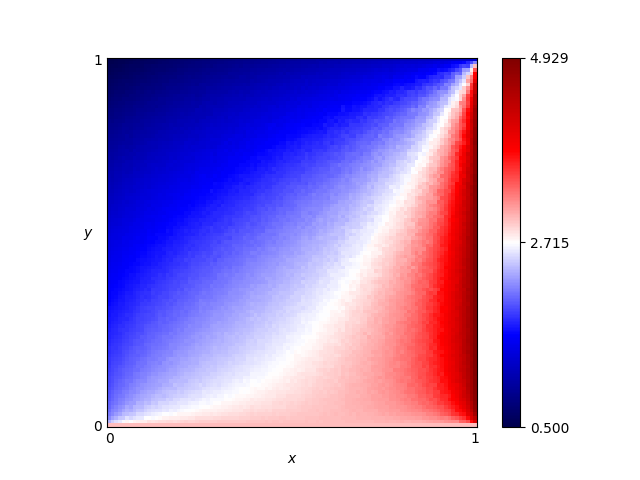
\includegraphics[height=.3\textheight]{./assets/images/Win-Stay_Lose-Shift.png}
    \caption{Pavlov fingerprinting with Tit for Tat used as the probe strategy.
    Figure was generated using~\cite{axelrodproject}.}
    \label{fig:fingerprinting}
\end{figure}

Due the nature of the research several pieces of software are starting to appear,
this includes a library called PRISON~\cite{prison}. PRISON is written in the
programming language Java and it has been used by it's authors in several
publications. The project includes a good number of strategies from the
literature but unfortunately the last update of the project dates back in 2004.

\subsection{Zero determinant (2012 - 2015)}

Following Section~\ref{section:modern_approaches}, this section is a review
of an important set of strategies, the zero determinant.

In~\cite{Press2012}, a new set of memory one strategies were introduced, called
\textbf{zero determinant (ZD)} strategies. The ZD strategies,
manage to force a linear relationship between the score of the strategy
and the opponent. Press and Dyson, prove their concept of the ZD strategies
and claim that a ZD strategy can outperform any given opponent.

The ZD strategies have attracted a lot of attention. It was stated that
``Press and Dyson have fundamentally changed the viewpoint on the Prisoner's
Dilemma''~\cite{Stewart2012}. In~\cite{Stewart2012}, a new tournament was
performed including ZD strategies and a new set of ZD
strategies the \textbf{Generous ZD}. Even so, ZD and memory one strategies have
also received criticism. In~\cite{Lee2015}, the `memory of a strategy does
not matter' statement was questioned. A set of more complex strategies,
strategies that take in account the entire history set of the game, were
trained and proven to be more stable than ZD strategies.

\subsection{Contemporary period (2015 - 2017)}

Following a discussion on research of short memory strategies this section
reviews recent work done in complex strategies. As well as a discussion of
new software and how modern approaches allows us to now revisit several pieces of
work produced in the past.

Modern approaches of artificial neural networks and machine learning are now used
in the field.  A number of strategies based on artificial neural networks are
introduced by~\cite{Knight2017}. Artificial neural networks provide a mapping
function to an action based on a selection of features computed from the history
of play.

These strategies are refereed to as \textbf{EvovlvedANN} strategies and are
based on a pre-trained neural network with the following features,

\begin{multicols}{2}
    \begin{itemize}
        \item Opponent's first move is C
        \item Opponent's first move is D
        \item Opponent's second move is C
        \item Opponent's second move is D
        \item Player's previous move is C
        \item Player's previous move is D
        \item Player's second previous move is C
        \item Player's second previous move is D
        \item Opponent's previous move is C
        \item Opponent's previous move is D
        \item Opponent's second previous move is C
        \item Opponent's second previous move is D
        \item Total opponent cooperations
        \item Total opponent defections
        \item Total player cooperations
        \item Total player defections
        \item Round number
    \end{itemize}
\end{multicols}

A representation of \textbf{EvovlvedANN 5} is given in Figure~\ref{fig:ann_5_neural}.
The inputs of the neural network are the 17 features as listed above. Number 5
reefers to the size of the hidden layer.

\begin{figure}[!hbtp]
    \centering
    \includestandalone[width=.5\textwidth]{./assets/tex/ann_5_neural}
    \caption{Neural network representation of EvovlvedANN 5.}
    \label{fig:ann_5_neural}
\end{figure}

In~\cite{Knight2017}, these representing methods are refereed to as archetypes.
Finite state machines and artificial neural networks are included in the
work but also new archetypes are introduced, such as hidden Markov models. A variant
of a finite state machine that use probabilistic transitions based on the prior
round of play to other states and cooperate or defect with various probabilities
at each state. Finite state machines and hidden Markov models
based strategies are characterized
by the number of states. Similarly, artificial neural networks based players
are characterized by the size of the hidden layer and number of input features.

Additionally a variant of a look up table is also presented called the lookerup
archetype. The lookerup archetype responses based on the opponent's first \(n_1\)
moves, the opponent's last \(m_1\) moves, and the players last \(m_2\) moves.
Taking into account the initial move of the opponent can give many insights.
For it is the only move a strategy is truly itself without being affected by
the other player. As a reminder, Axelrod in his work
highlighted the importance of the initial move and believed that it was one
of the secrets of success of the strategy Tit for Tat.

Finally, a new archetype called the Gambler is also introduced, which is a
stochastic variant of the lookerup archetype.

Archetypes are used with evolutionary algorithms to train set of
new strategies. The evolutionary algorithm used in both~\cite{Axelrod1987,
Gaudesi2016} is called genetic algorithm. Other algorithms including particle
swarm optimization have been used in research of the most dominant strategy
\cite{Franken2005}.

In~\cite{Knight2017} the approach in used to introduce as stated
by the authors the best performing strategies for the iterated prisoner's dilemma.
These strategies will be refereed  as \textbf{Evolved} strategies.
Several successful new strategies are,

\begin{itemize}
    \item \textbf{EvolvedLookerUp2\_2\_2} a looker up strategy trained with a
    genetic algorithm; EvolvedLookerUp2\_2\_2 responses based on the opponent's
    2 first and last moves and the player's 2 last moves. Thus \(n_1=2, m_1=2\)
    and \(m_2=2\).
    \item \textbf{Evolved HMM 5} a 5 states hidden markov model trained with a genetic
    algorithm;
    \item \textbf{Evolved FSM 16} a 16 state machine trained with a genetic
    algorithm;
    \item Finally \textbf{PSO Gambler 2 2 2} a looker up strategy trained with
    a particle swarm algorithm, where \(n_1=2, m_1=2\) and \(m_2=2\).
\end{itemize}

Though several papers have claimed before to have discovered the dominant
strategies for the game the work of \cite{Knight2017} is promising.
This is due the fact that the introduced strategies have been trained using
different types of evolutionary algorithms in a pool of 176 well known
strategies for the literature. Including all the strategies that have been
discussed in this section.

This was made possible due an open source  library, called the Axelrod project
\cite{axelrodproject}. The project is written in the programming language
Python, it is accessible and open source. To date the list of strategies implemented
within the library exceed the 200. The project has been used in several
publications including~\cite{Knight2017} and a paper describing it and
it's capabilities was published in 2016~\cite{Knight2016}. The source code
for Tit for Tat as implement within the library is shown in Figure
\ref{fig:tit_for_tat_axelrod}. Furthermore, performing a tournament
with a selection of strategies is possible in five lines of code, shown in
Figure~\ref{fig:tournament_code}.

\begin{figure}[!hbtp]
    \centering
    \begin{minted}
        [
        autogobble=true,
        framesep=2mm,
        fontsize=\normalsize,
        ]
        {python}
def strategy(self, opponent: Player) -> Action:
    """This is the actual strategy"""
    # First move
    if not self.history:
        return C
    # React to the opponent's last move
    if opponent.history[-1] == D:
        return D
    return C
    \end{minted}
    \caption{\label{fig:tit_for_tat_axelrod} Source code for Tit for Tat in Python
    as implemented in Axelrod Python library~\cite{axelrodproject}}.
\end{figure}

\begin{figure}[!hbtp]
    \centering
    \begin{minted}
        [
        autogobble=true,
        framesep=2mm,
        fontsize=\normalsize,
        ]
        {python}
>>> import axelrod as axl
>>> players = (axl.Cooperator(), axl.Defector(), axl.TitForTat(), axl.Grudger())
>>> tournament = axl.Tournament(players)
>>> results = tournament.play()
>>> results.ranked_names
['Defector', 'Tit For Tat', 'Grudger', 'Cooperator']
    \end{minted}
    \caption{\label{fig:tournament_code} Performing a computer tournament
    using~\cite{axelrodproject}.}
\end{figure}

Software has a crucial role in research. Well written and maintained software
allows the reproducibility of prior work and can accelerate findings within the
field. The field of the iterated prisoner's dilemma has suffered the consequences
of poor research software. As stated above the source code of the initial
computer tournament is not retrievable. Several of the strategies that competed
in the tournament are not given a full explanation of how the decided on their
next move. In terms of best practice and reproducibility the Axelrod library
is the lead software in the field.

Other recent projects include~\cite{pd_trust, pd_game}, both are education
platforms and not research tools. In~\cite{pd_trust}, several concepts such as
the iterated game, computer tournaments and evolutionary dynamics are introduced
through a user interface game. Project~\cite{pd_game} offers a big collection of
strategies and allows the user to try several match and tournaments configurations.
Such as noise.

In~\cite{Rapoport2015}, the authors claim that they have managed to
re-run the first tournament that Axelrod performed. They tried to push his work
further by altering aspects such as, the format of the tournament, the objective
and the population. One of the authors claimed to have been a contributor
to the first tournaments, which would explain how it was managed to reproduce
the tournament.

\subsubsection{Biological Applications}
%TODO include the cancer studies.
\begin{itemize}
    \item \cite{Turner1999} uses evolutionary game theory to study the spread of
    virus.
    \item \cite{Douglas2011} a shout for his work, using tit for tat to study cells.
\end{itemize}

\section{Data Analysis}\label{section:analysis}

In this section we will focus on the analysis of the study of the prisoner's dilemma
using a large dataset of articles. This data set will be used to ascertain the level
of collaborative nature of the field and identify influencers. This will be done
relative to:

\begin{itemize}
    \item Other sub fields of game theory: auction games~\cite{menezes2005} and 
    the price of anarchy~\cite{roughgarden2005}.
    \item A temporal analysis.
\end{itemize}

\subsection{Data Collection}

Before analysing our data in this subsection we will describe the data collection
process.

Academic articles are accessible through scholarly databases and collections of
academic journals. Several databases and collections today offer access through
an open application protocol interface (API). An API allows users to query
directly a journal's database and skip the user interface side of the journal.
Interacting with an API has two phases:

\begin{enumerate}
    \item requesting;
    \item receiving;
\end{enumerate}

The request phase includes composing a url with the request. Figure~\ref{fig:request_message}
demonstrates an example request. The first part of the request is the address of
the API we are querying. In this example the address is that of the arXiv API.
The second part of the request contains the search arguments. In our example we
are requesting for a single article that the word `prisoners dilemma' exists within
it's title. The format of the request message is different from API to API.

The receive phase includes receiving a number of raw metadata of articles that
satisfied the request message. The raw metadata are commonly received in a xml
or a json format~\cite{nurseitov2009}. Similarly to the request message, the
structure of the received data differs from journal to journal.

\begin{figure}[!hbtp]
    \centering
    \begin{minted}
        [
        autogobble=true,
        framesep=2mm,
        fontsize=\normalsize,
        ]
        {xml}
        http://export.arxiv.org/api/query?search_query=abs:prisoner's dilemma&max_results=1
    \end{minted}
    \caption{\label{fig:request_message} A request message for the arXiv API.}
\end{figure}

The data collection is crucial to this study, to ensure that this study can be
reproduced all code used to query the different APIs has been packaged and is
available online~\cite{nikoleta_2017}. The software could be used for any type of
project similar to the one described here, documentation for it is available at:
\url{http://arcas.readthedocs.io/en/latest/}.

The following sources were used to collect data,
\begin{enumerate}
        \item arXiv~\cite{mckiernan2000};
        \item PLOS~\cite{plos_one};
        \item IEEE;
        \item Nature;
        \item Springer.
\end{enumerate}

These are four prominent journals in the field, as well as the arXiv~\cite{mckiernan2000}
pre print server. In the case of an article being both in a journal and the arXiv,
only the journal version was considered.

For each article~\cite{nikoleta_2017} collects a list of the features, shown in Table~\ref{table:arcas_results}.
Note that the plain text of the article is not collected, just the metadata. The
data is archived and available at. %TODO: archive data
In this work only the features of Table~\ref{table:result_set} are used.

\begin{table}[!hbtp]
    \begin{center}
    \resizebox{0.9\linewidth}{!}{\arraycolsep=2.5pt%
        \begin{tabular}{lll}
            \toprule
             & Result name & Explanation \\
             \midrule
             1 & Abstract & The abstract of the article.\\ 
             2 & Author & A single entity of an author from the list of
             authors of the respective article.\\ 
             3 & Date & Year of publication.\\ 
             4 & Journal & Journal of publication.\\ 
             5 & Key & A generated key containing an authors name and
             publication year (ex. Glynatsi2017).\\ 
             6 & Keyword & A single entity of a keyword assigned to the article
             by the given journal.\\ 
             7 & Labels & A single entity of labels assigned to the article
             manual by us.\\ 
             8 & Pages & Pages of publication.\\ 
             9 & Provenance & Scholarly database for where the article was
             collected.\\ 
             10 & Score & Score given to article by the given journal.\\ 
             11 & Title & Title of article.\\ 
             12 & Unique key &  A unique key. \\ 
            \bottomrule
        \end{tabular}}
    \end{center}
    \caption{Metadata for each entry/article.}
    \label{table:arcas_results}
\end{table}

\begin{table}[!hbtp]
    \begin{center}
        \begin{tabular}{lll}
            \toprule
             & Result name & Explanation \\
             \midrule
             1 & Abstract & The abstract of the article.\\ 
             2 & Author & A single entity of an author from the list of
             authors of the respective article.\\ 
             3 & Date & Year of publication.\\ 
             4 & Journal & Journal of publication.\\ 
             5 & Provenance & Scholarly database for where the article was
             collected.\\ 
             6 & Title & Title of article.\\ 
            \bottomrule
        \end{tabular}
    \end{center}
    \caption{Structure of data set. Contained results.}
    \label{table:result_set}
\end{table}

In the work described here, a series of keywords were used to identify relevant
articles. Articles for which these keywords were in the title or the abstract
are included in the analysis. A list of the keywords that were used are
shown in Table~\ref{table:search_keywords}.

\begin{table}[!hbtp]
    \begin{center}
        \begin{tabular}{lll}
            \toprule
             & Keywords & \\
            \midrule
             1 &  prisoner's dilemma & \\
             2 &  prisoners dilemma  & \\
             3 &  tit-for-tat & \\
             4 &  tit for tat & \\
             5 &  zero determinant strategies & \\
            \bottomrule
        \end{tabular}
    \end{center}
    \caption{Keywords used in searching for articles.}
    \label{table:search_keywords}
\end{table}

Similarly, for collecting data on auction games and the price of anarchy the
following keywords respectively for each topic,

\begin{itemize}
    \item key: auction game theory;
    \item key: price of anarchy.
\end{itemize}

\subsection{Preliminary Analysis}

A total of three data sets are explored in this work. A summary of each data is
presented in this section. The three data sets are,

\begin{itemize}
    \item the main data set which contains articles on the prisoner's dilemma,~\cite{}
    \item a secondary data set which contains article on auction games~\cite{} and
    \item a secondary data set which contains articles on the price of anarchy~\cite{}.
\end{itemize}
% TODO archive all data sets

\paragraph{The prisoner's dilemma data set}
\mbox{ }\\

The main data set and the main focus of this analysis. The data set~\cite{}
consists of \totalarticles articles, where \uniquetitles have unique titles.
%TODO add reference to archived dataset
This is because a total of \numberofduplicates articles have been collected from
both a journal and arXiv. All duplicates from arXiv are dropped, thus hereupon
we consider \uniquetitles unique article entries.

There are a number of \manual articles that have not been collected from the
aforementioned APIs. These articles were manually added to the dataset throughout
the writing of Section~\ref{section:timeline}. A more detailed summary of the 
articles' provenance is given by Table~\ref{table:provenance}.

\begin{table}[!hbtp]
    \begin{center}
    \begin{tabular}{lrr}
\toprule
{} &  \# of Articles &  Percentage \\
provenance &                &             \\
\midrule
Manual     &             89 &        2.92 \\
IEEE       &            295 &        9.67 \\
Springer   &            458 &       15.01 \\
PLOS       &            482 &       15.79 \\
Nature     &            673 &       22.05 \\
arXiv      &           1055 &       34.57 \\
\bottomrule
\end{tabular}

    \end{center}
    \caption{Articles' provenance for~\cite{}.}
    \label{table:provenance}
\end{table}

The larger number of articles were collected from arXiv, Springer and IEEE. Both
Nature and PLOS have a small contribution to the size of the data set. The oldest
article was published in 1944 and the most recent one in 2017. Note
that the last data collection was on December 2017.
% TODO Ensure this stay accurate

Moreover we calculate the average publication over time. This is done for the overall
data set and for each journal individually. The average publication is estimated
as the ratio of the number of articles and the years of publication. Denoted as
\(\mu_p\),

\[ \mu_p = \frac{N_a}{N_y}\]

where \(N_a\) is number of articles and \(N_u\) is the years of publication.

The years of publication is calculated as the range between 2017 and the first published
article within the data.

Table~\ref{table:publication_rates} summarises these averages. Overall an average of
21 articles are published per year on the topic. The most significant contribution
to this appears to be from arXiv with 8 articles per year, followed by Springer
with 5 articles per year.

\begin{table}[!hbtp]
    \begin{center}
    \begin{tabular}{lr}
\toprule
{} &  Av. Yearly publication \\
\midrule
IEEE     &                     5.0 \\
PLOS     &                     8.0 \\
Springer &                     9.0 \\
Nature   &                    11.0 \\
arXiv    &                    16.0 \\
Overall  &                    49.0 \\
\bottomrule
\end{tabular}

    \end{center}
    \caption{Average publication for~\cite{}.}
    \label{table:publication_rates}
\end{table}

% The trends of these rates can also be explored. This is achieved by using the 
% software package Prophet by Facebook. Prophet fits an additive model
% to the data. The results are demonstrated in Figure~\ref{fig:provenance}.
% It seems that all journals have an increasing trend, apart from Nature which has
% a constant number of publications throughout the years.

% \begin{figure}[!hbtp]
%     \centering
%     \begin{subfigure}{.4\textwidth}
%         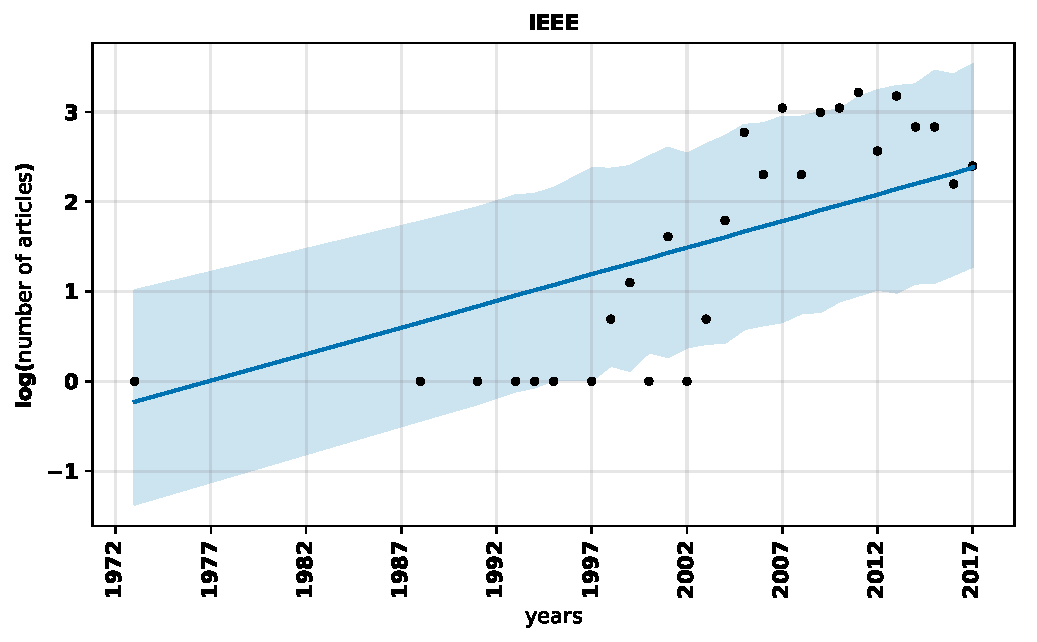
\includegraphics[width=\textwidth]{./assets/images/trend_IEEE.pdf}
%     \end{subfigure}
%     \begin{subfigure}{.4\textwidth}
%         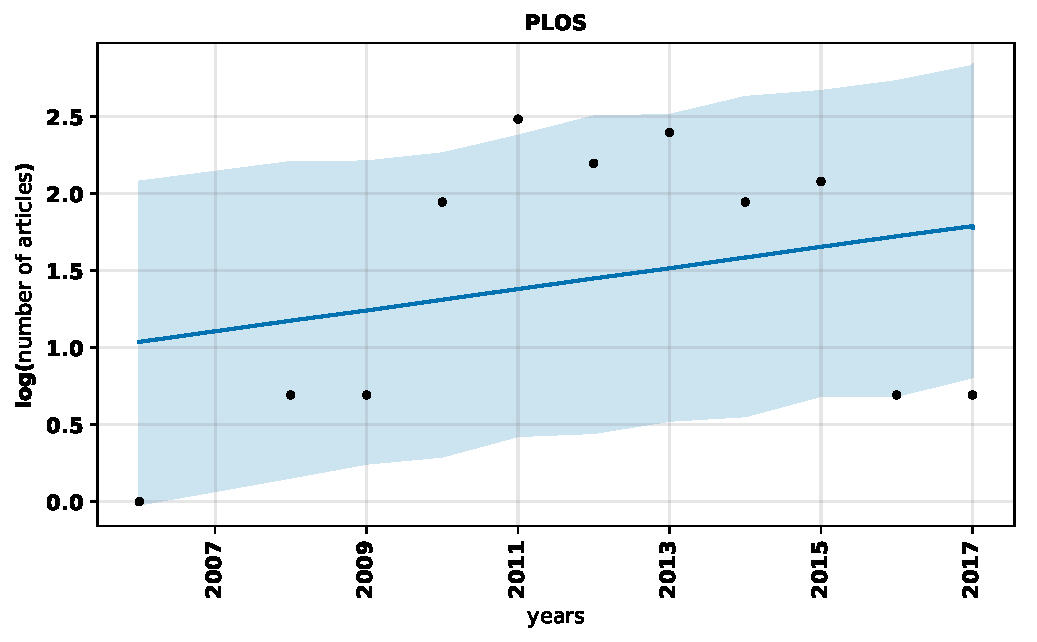
\includegraphics[width=\textwidth]{./assets/images/trend_PLOS.pdf}
%     \end{subfigure}
%     \begin{subfigure}{.4\textwidth}
%         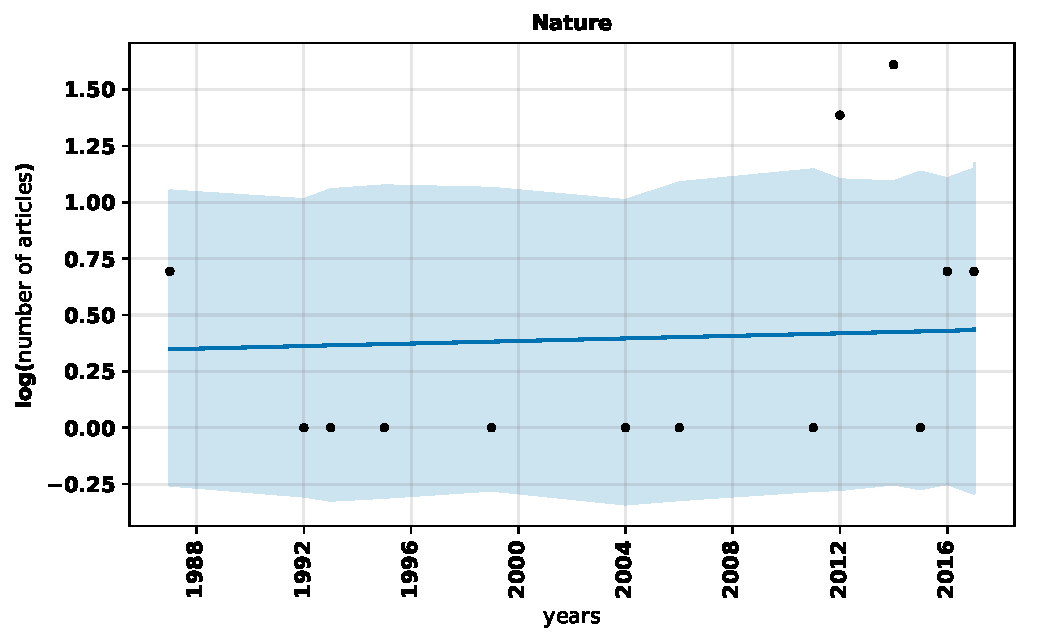
\includegraphics[width=\textwidth]{./assets/images/trend_Nature.pdf}
%     \end{subfigure}
%     \begin{subfigure}{.4\textwidth}
%         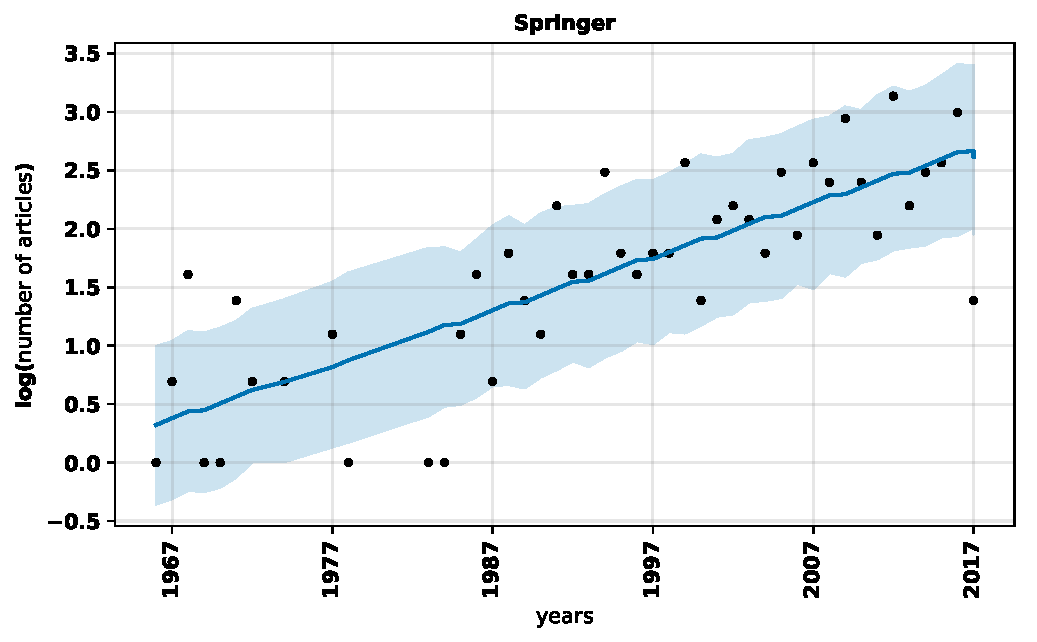
\includegraphics[width=\textwidth]{./assets/images/trend_Springer.pdf}
%     \end{subfigure}
%     \begin{subfigure}{.4\textwidth}
%         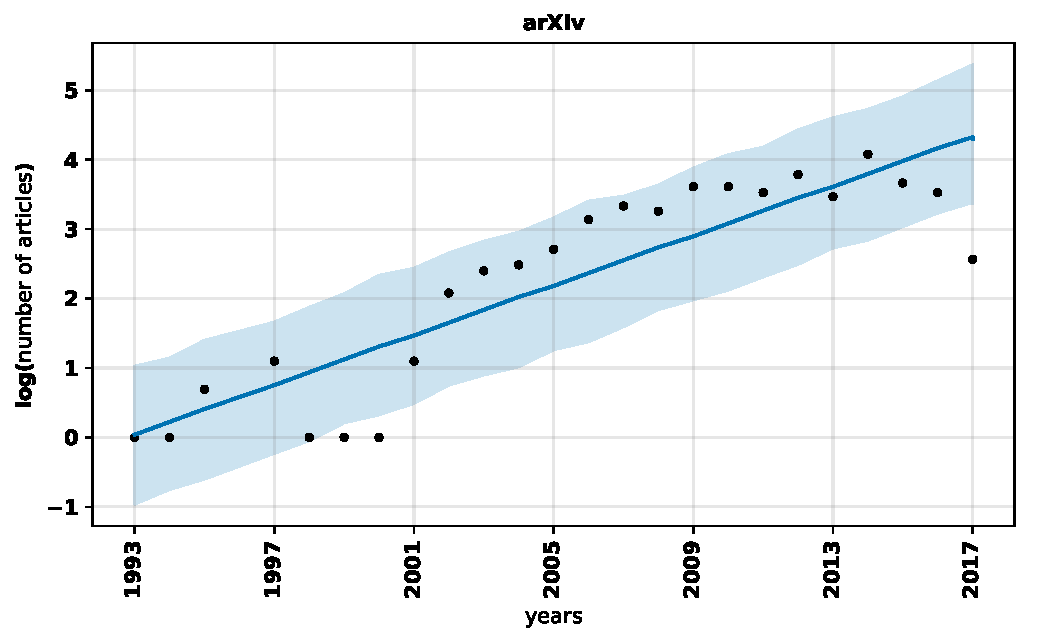
\includegraphics[width=\textwidth]{./assets/images/trend_arXiv.pdf}
%     \end{subfigure}
%     \caption{Number of publications over time for each journal.}
%     \label{fig:provenance}
% \end{figure}

\paragraph{Auction games and the price of anarchy data sets}
\mbox{ }\\

A summary of both data sets, auction games~\cite{} and price of anarchy~\cite{},
is given by Table~\ref{table:summary_other_topics}.

A total of 2103 articles with 3860 unique authors are examined for auction games.
Auction games is well studied topic with the earliest entry going
back to 1974. In comparison, 296 unique articles have been collected on price of
anarchy. The earliest entry being in 2003 and a total of 668 unique authors have
written about the topic.

In Figure~\ref{fig:timeplots_other_topics} a time plot for each topic is
displayed and is exhibited that both topics have had an increasing trend over
the years. Though price of anarchy is clearly a new topic compared to auction games.

The frequency of the prisoner's dilemma, for both articles and authors, lies
between the frequencies of these two topics.

\begin{table}[!hbtp]
    \begin{center}
    \begin{tabular}{llr}
        \toprule
         &            Price of anarchy &  Auction games \\
        \midrule
        Unique articles      & 296  & 2103 \\
        Unique authors       & 668  & 3860 \\
        Min publication year & 2003 & 1974 \\
        Max publication year & 2017 & 2017 \\
        \bottomrule
    \end{tabular}
    \end{center}
    \caption{Data sets~\cite{} and~\cite{} summary.}
    \label{table:summary_other_topics}
\end{table}

\begin{center}
\begin{figure}[!hbtp]
    \begin{subfigure}{0.5\textwidth}
        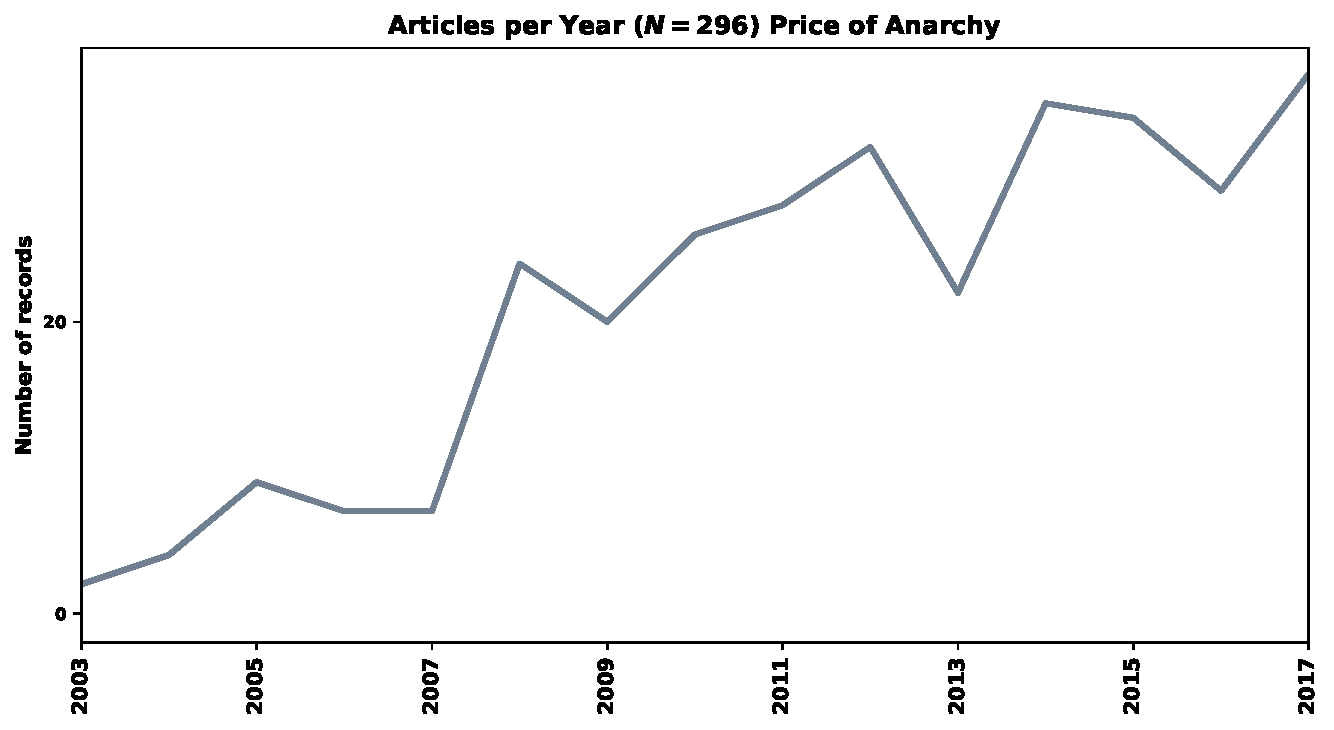
\includegraphics[width=\textwidth]{./assets/images/anarchy_timeline.pdf}
    \end{subfigure}
    \begin{subfigure}{0.5\textwidth}
        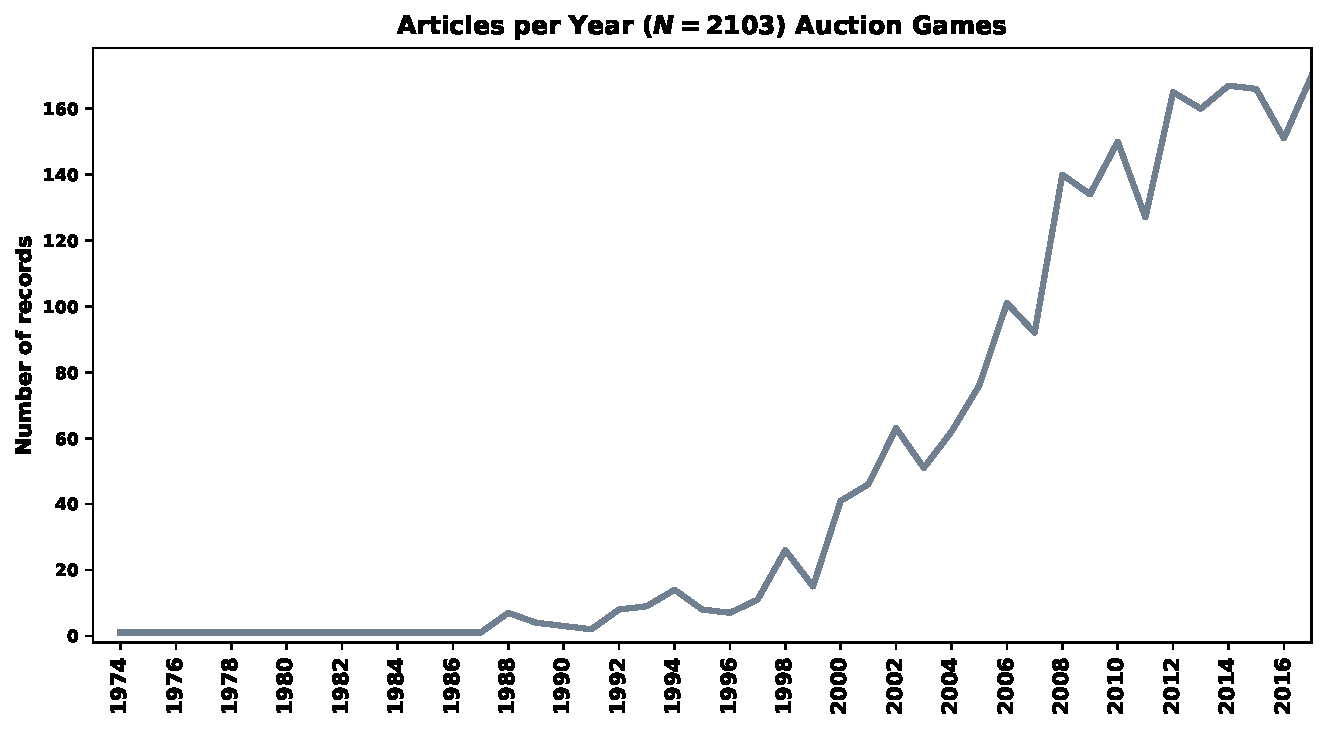
\includegraphics[width=\textwidth]{./assets/images/auction_timeline.pdf}
    \end{subfigure}
\caption{Time plots of~\cite{} and~\cite{}.}
\label{fig:timeplots_other_topics}
\end{figure}
\end{center}

The provenance of the articles is given by Table~\ref{table:provenance_other_topics}.
Almost 1500 article for auction games have been collected from Springer, that is
more than three times the articles that have been collected from other sources.
PLOS and Nature have a minor contribution and PLOS and Nature had no
articles on the price of anarchy.

\begin{table}[!hbtp]
    \begin{center}
    \begin{tabular}{lcc}
        \toprule
        \textbf{Provenance} & \textbf{Total articles} & \textbf{Total articles}\\
                   & (auction games) & (price of anarchy)\\
        \midrule
        Springer   &                1429 &                78 \\
        arXiv      &                 436 &                108 \\
        IEEE       &                 301 &                131 \\
        PLOS       &                  15 &                 -  \\
        Nature     &                   1 &                 -   \\
        \bottomrule
    \end{tabular}
    \end{center}
    \caption{Articles' provenance for~\cite{} and ~\cite{}.}
    \label{table:provenance_other_topics}
\end{table}

\begin{table}[!hbtp]
    \begin{center}
    \begin{tabular}{lcc}
        \toprule
        \textbf{Provenance} & \textbf{Av. publication}  & \textbf{Av. publication}\\
                            & (auction games) & (price of anarchy)\\
        \midrule
        Overall             &          58.973 & 19.812 \\
        Springer            &          38.622 & 4.875  \\
        arXiv               &          11.784 & 6.750   \\
        IEEE                &           8.135 & 8.188    \\
        PLOS                &           0.405 &   -       \\
        Nature              &           0.027 &   -        \\
        \bottomrule
    \end{tabular}
    \end{center}
    \caption{Average publication for auction games and the price of anarchy.}
    \label{table:other_topics_publication_rates}
\end{table}

The overall average publication for~\cite{} and~\cite{} are 59 and 20 articles
respectively. It appears that auction games publication is largely different
for both the prisoner's dilemma and the price of anarchy. These two topics have
the same average publication. Note that the significance of each journal differs
from topic to topic. Though this analysis will not focus on individual sources
from hereupon.

\paragraph{Temporal analysis}
\mbox{ }\\

For comparison reasons in the following subsections the analysis will also be
held relative to a temporal analysis. The main data set~\cite{}
is divided into time period according to the subsections of Section~\ref{section:timeline}.
The respective measures of unique titles and unique authors for each period is
given by Table~\ref{table:summary_temporal}.

\begin{table}[!hbtp]
    \begin{center}
    \begin{tabular}{lrr}
\toprule
{} &  \textbf{Unique articles} &  \textbf{Unique authors} \\
\midrule
period 1: (1961 - 1972) &               21 &              38 \\
period 2: (1981 - 1984) &                5 &               6 \\
period 3: (1984 - 1993) &               64 &              70 \\
period 4: (1987 - 1999) &              121 &             169 \\
period 5: (1995 - 2015) &              926 &            1730 \\
period 6: (2012 - 2017) &              453 &            1008 \\
period 7: (2015 - 2017) &              180 &             466 \\
\bottomrule
\end{tabular}

    \end{center}
    \caption{Periods and their respective measures.}
    \label{table:summary_temporal}
\end{table}

In this section we have described the three data sets that we are going to use
in the following sections in order to identify collaborative behaviour and influence.
Two data sets of different topics are used for comparison reasons. The frequency of
articles and authors differs within the three data sets which is ideal. Furthermore
the journals effect also differ but not much will be done at that level form now
onwards.

Finally a temporal analysis of the data sets~\cite{} will also assists us in
obtaining more insights. The period have also be presented here.
In the following section we explore the authors of the papers and their
connections to one another.

\subsection{Co authorship Analysis}

% TODO Describe some works that look at literature graphs (these typically look
% at citation graphs)
% TODO Describe how these are often used to measure influence however (mention
% that blog post) influence does not correspond to citation.
% TODO Define the co author network as a weight graph G =...
% TODO Possibly include subgraphs as examples.

Measuring academic collaborations and the influence academics offer to their
field is not always trivial. Several studies consider academic citations as a measure
and base their analysis on the citations network. According to a blog post~\cite{nature_blog} 
written by Nature in 2017, depending on citations can often be misleading.
This is because:

\begin{itemize}
    \item The true number of citations can not be known. Citations can be missed
    due data entry errors or typos in a journal.
    \item Academics are influenced by many more papers than they actually cite.
    \item Several citations are superficial.
\end{itemize}

We are in agreement with the aforementioned reasons and in this work citations
will not be considered. On the contrary we introduce an alternative way of measuring
both \textbf{collaborative behaviour} and \textbf{influence} based on the co authorship network.
Initially we discuss how such network can be constructed for a given topic and
then we consider several network measures to retrieve our results. 
%TODO write more here
Measures such as,

\begin{itemize}
    \item the number of connected components,
    \item clustering coefficient,
    \item degrees distributions and
    \item centrality measures.
\end{itemize}

All network measures are introduced with examples in the following sections.

\subsubsection{Constructing a co authorship network}

To construct a co authorship network we need to consider all the unique authors of a data set.
The issue with retrieving the unique authors is that authors names can be written
in different ways in different sources. For example consider the author of this
paper:

\begin{itemize}
    \item Nikoleta Glynatsi
    \item Nikoleta E. Glynatsi
    \item Nikoleta Evdokia Glynatsi
\end{itemize}

Consequently, several different entries of the same author existed within the data
set. To address the problem the Levenshtein Distance~\cite{miller2009} was used.
The Levenshtein Distance is a metric for measuring the difference between two
sequences. The Levenshtein distance between two strings is defined as the
minimum number of edits needed to transform one string into the other, with the
allowable edit operations:

\begin{enumerate}
    \item insertion;
    \item deletion;
    \item substitution of a single character.
\end{enumerate}

The ration of the Levenshtein distance of all possible pairs of authors in the
data set was computed. If the ratio was between \(85\) and \(99\) the entries were
highlighted. The highlighted entries were manually checked to assure that there
were indeed the same author and then one of them was replaced by the other.
%Example

For example all entries with author name written as example 1 were replaced by
2.

\begin{enumerate}
    \item Y. Moreno
    \item Yamir Moreno
\end{enumerate}

The manual check is performed because not all highlighted entries are indeed the
same. For example:

\begin{enumerate}
    \item Zhen Yang and
    \item Zhen Wang
\end{enumerate}

are two different authors.

Once we have cleaned the name entries the number of unique authors is calculated.
%Define what a network is and then G_1, G_2, G_3
The co authorship network of the prisoner's dilemma can now be defined as:

An undirected graph \(G\) of vertices \(V\) and edges \(E\), Figure~\ref{fig:authors_network}.
There are \authors vertices representing each unique author. The vertices are
joined by \edges edges. An edge connects two authors if and only if those authors
have written together. No weight has been applied to the edges nor the nodes.

\begin{figure}[!hbtp]
    \centering
    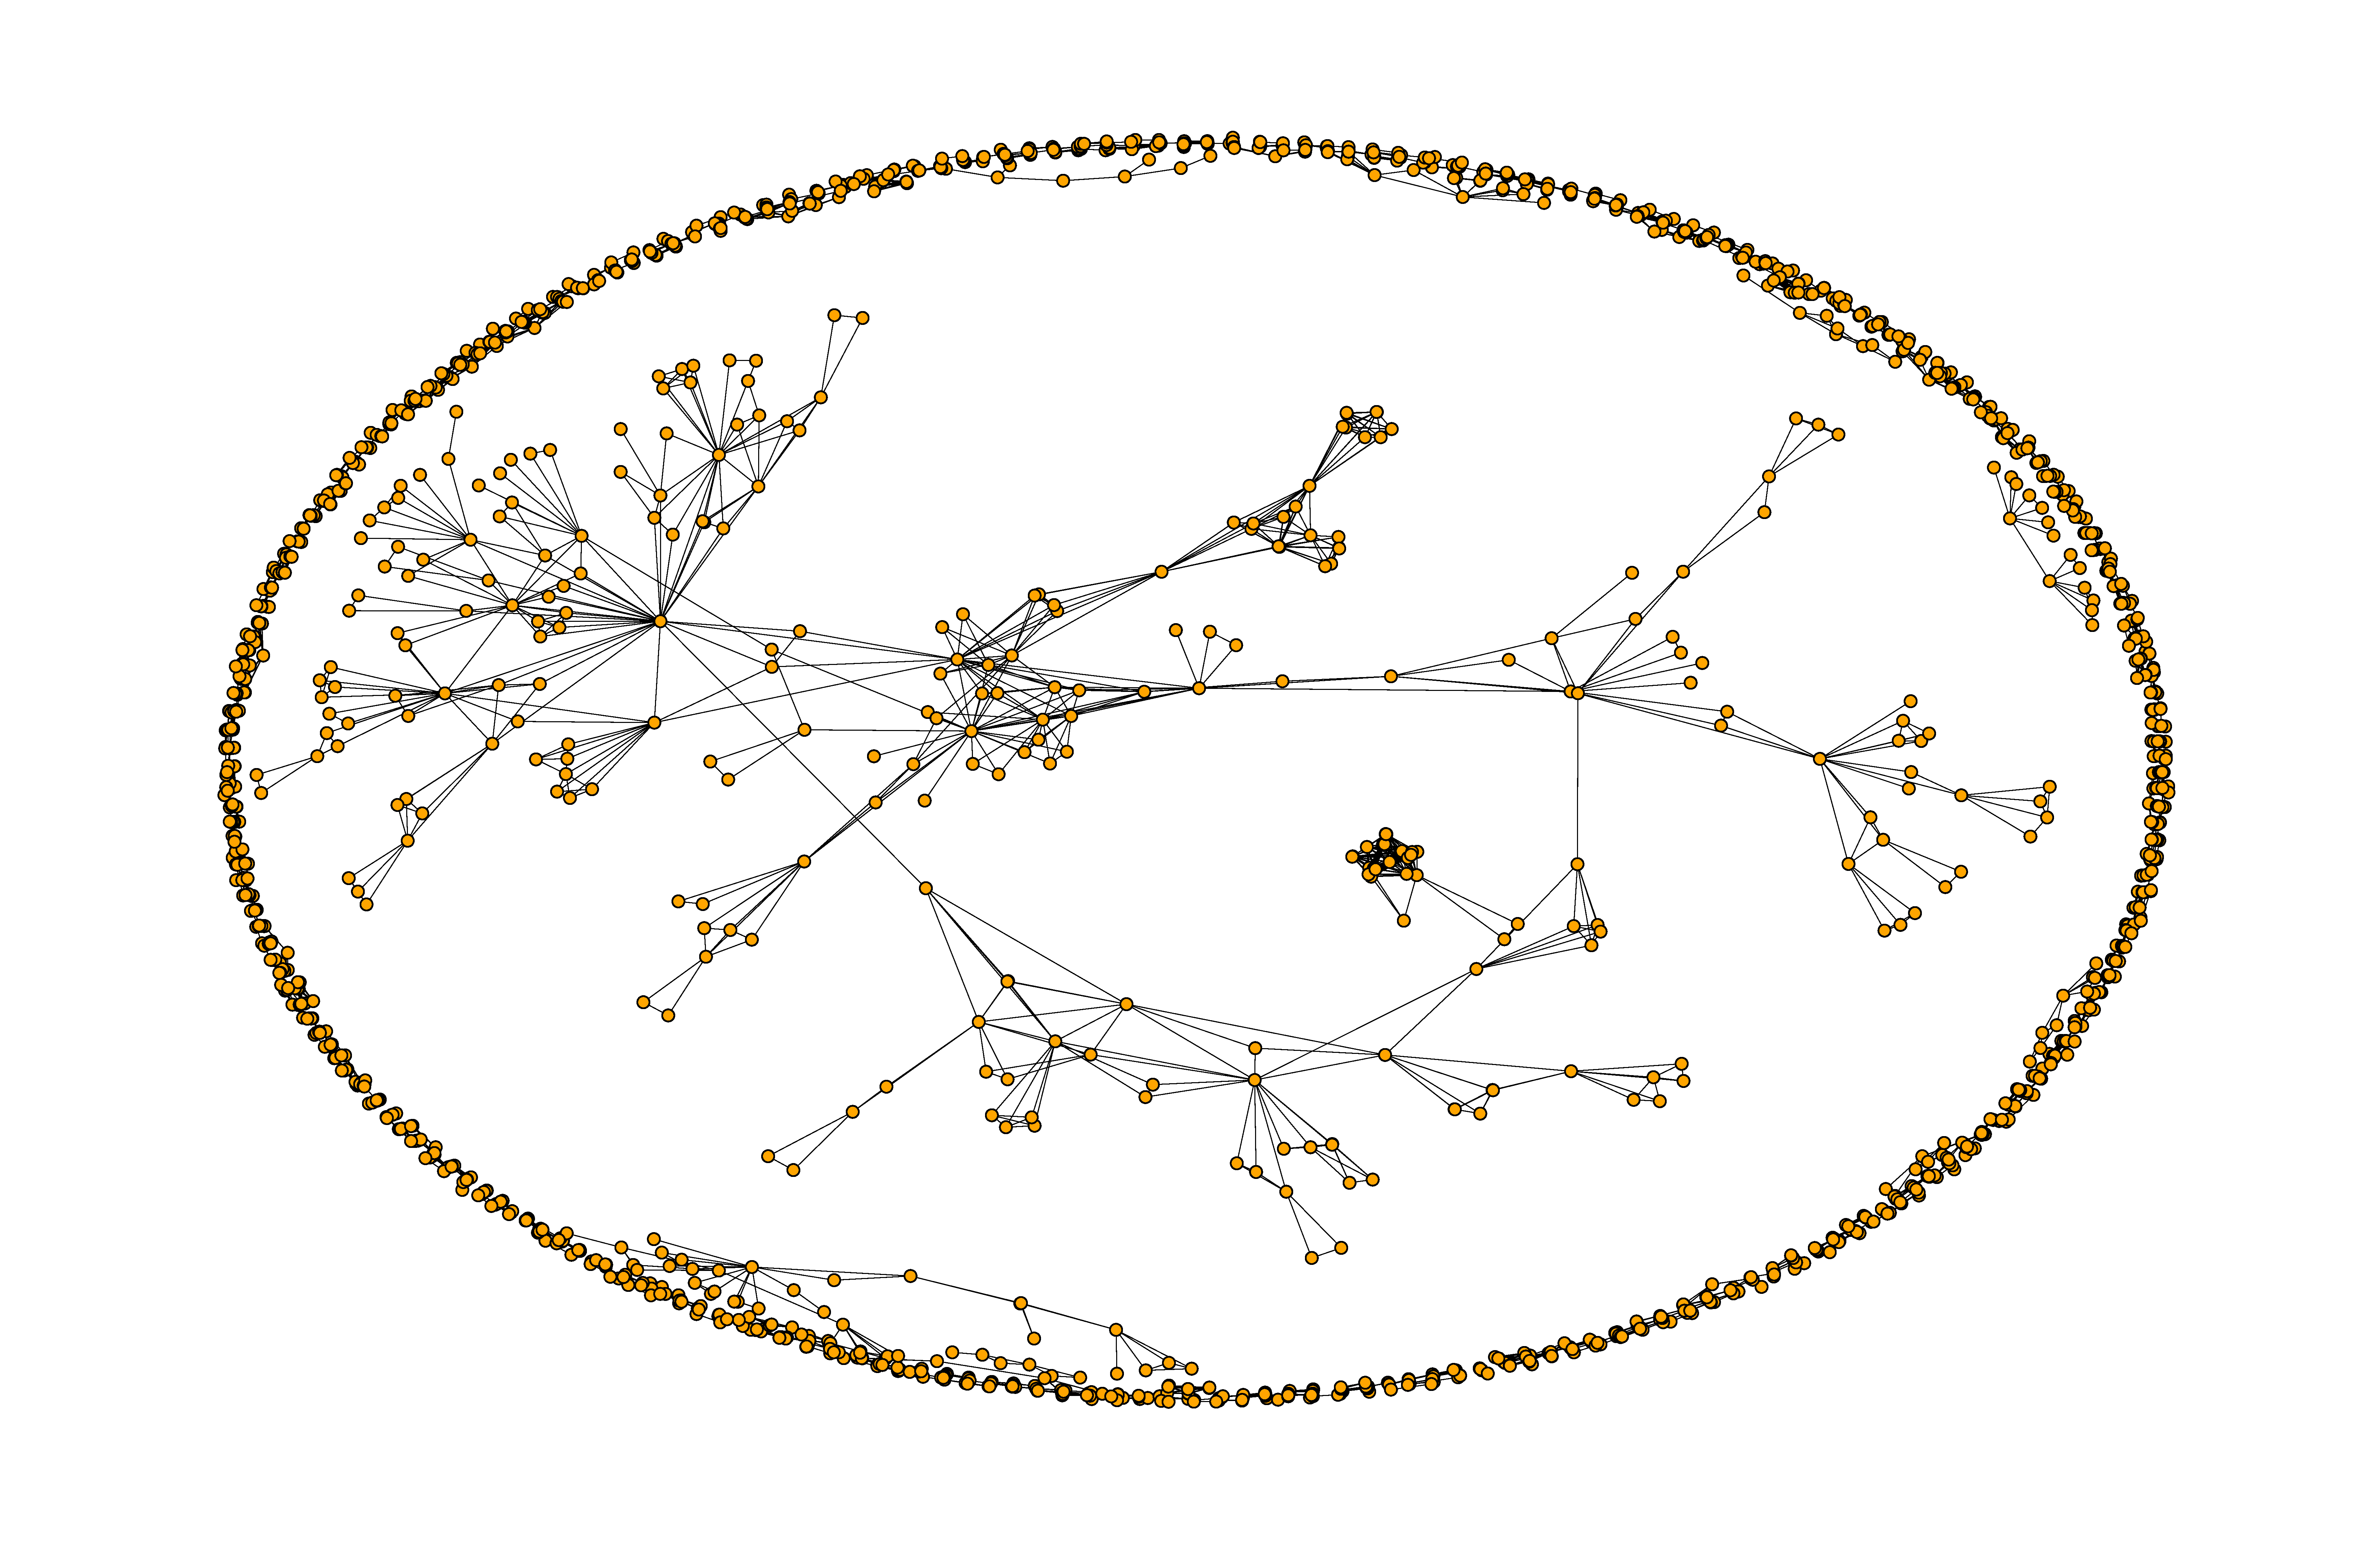
\includegraphics[width=0.8\textwidth]{./assets/images/co-authors-network.pdf}
    \caption{Co authorship network for prisoner's dilemma.}\label{fig:authors_network}
\end{figure}

The same approached is used to construct the networks for auction games and the
price of anarchy. For auction games there are \auctionauthors vertices and \auctionedges
edges. The price of anarchy corresponds to a smaller network with \priceauthors
vertices and \priceedges edges. Their respective networks are illustrated in
Figure~\ref{fig:co-authorship-other-topics}. The following sections focuses on
the analysis of these networks.

\begin{center}
    \begin{figure}[!hbtp]
        \begin{subfigure}{0.5\textwidth}
            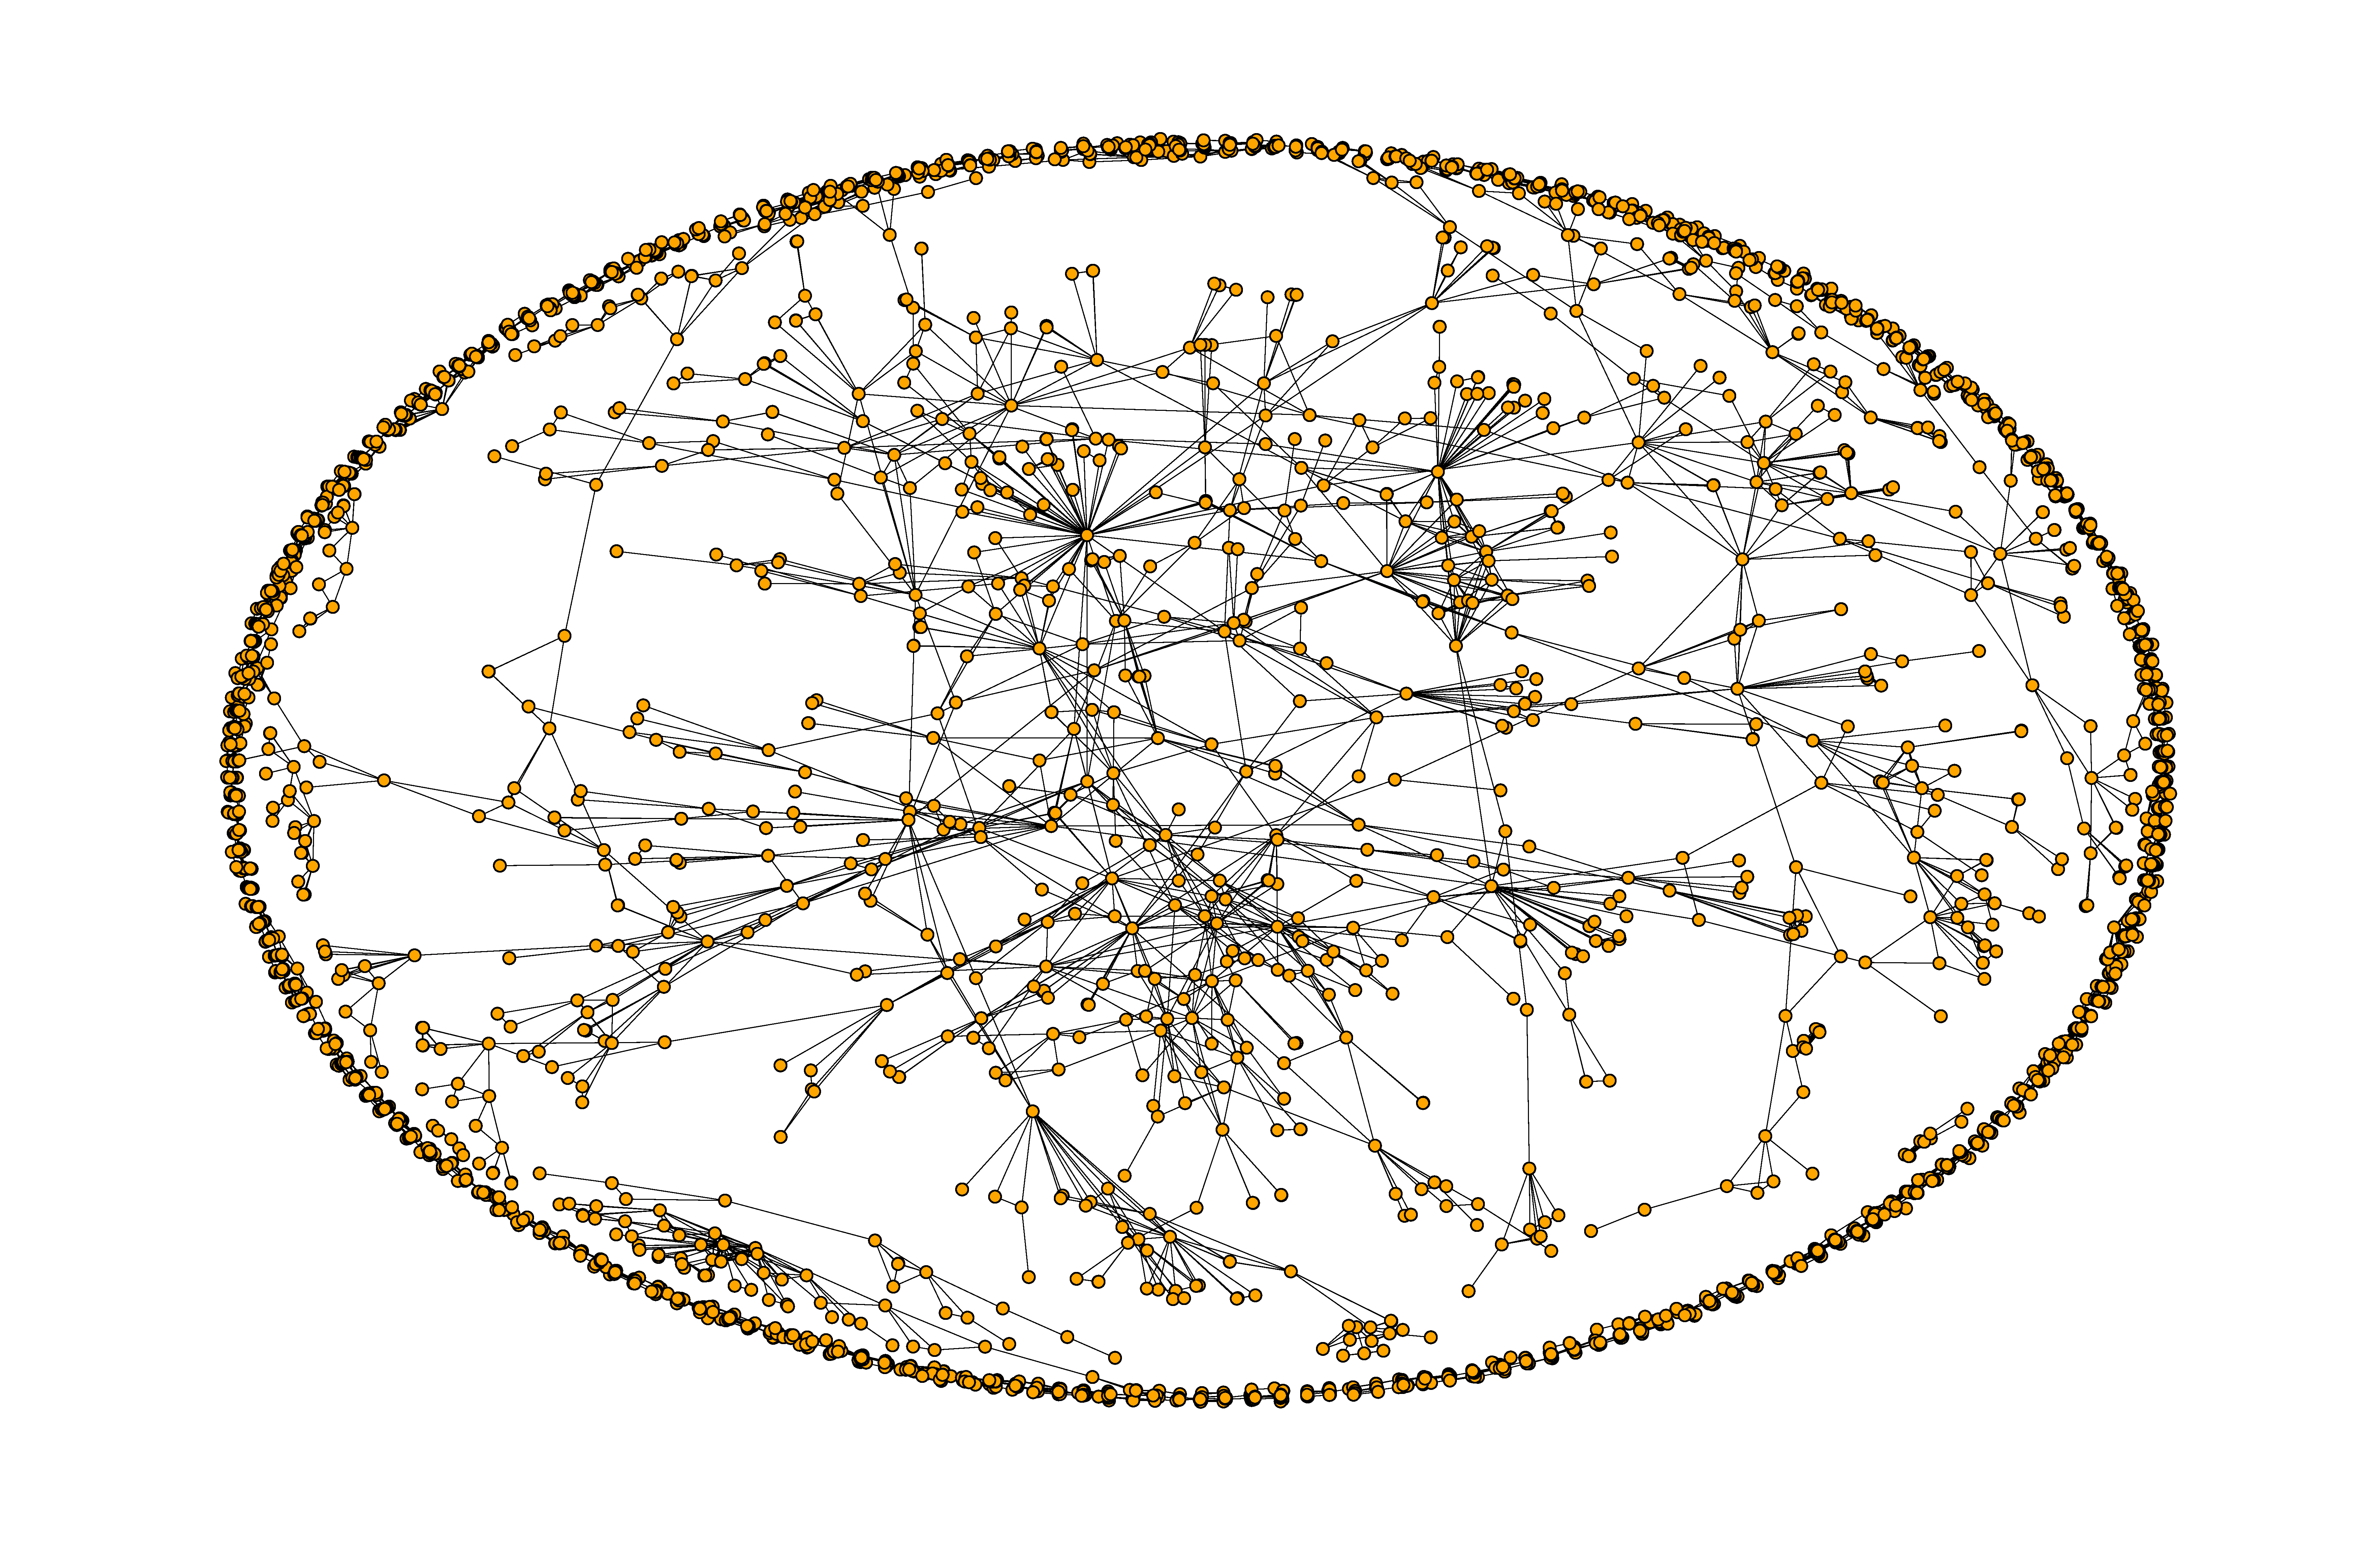
\includegraphics[width=\textwidth]{./assets/images/co-authors-network-auction.pdf}
            \caption{Co authorship network for auction games.}
        \end{subfigure}
        \begin{subfigure}{0.5\textwidth}
            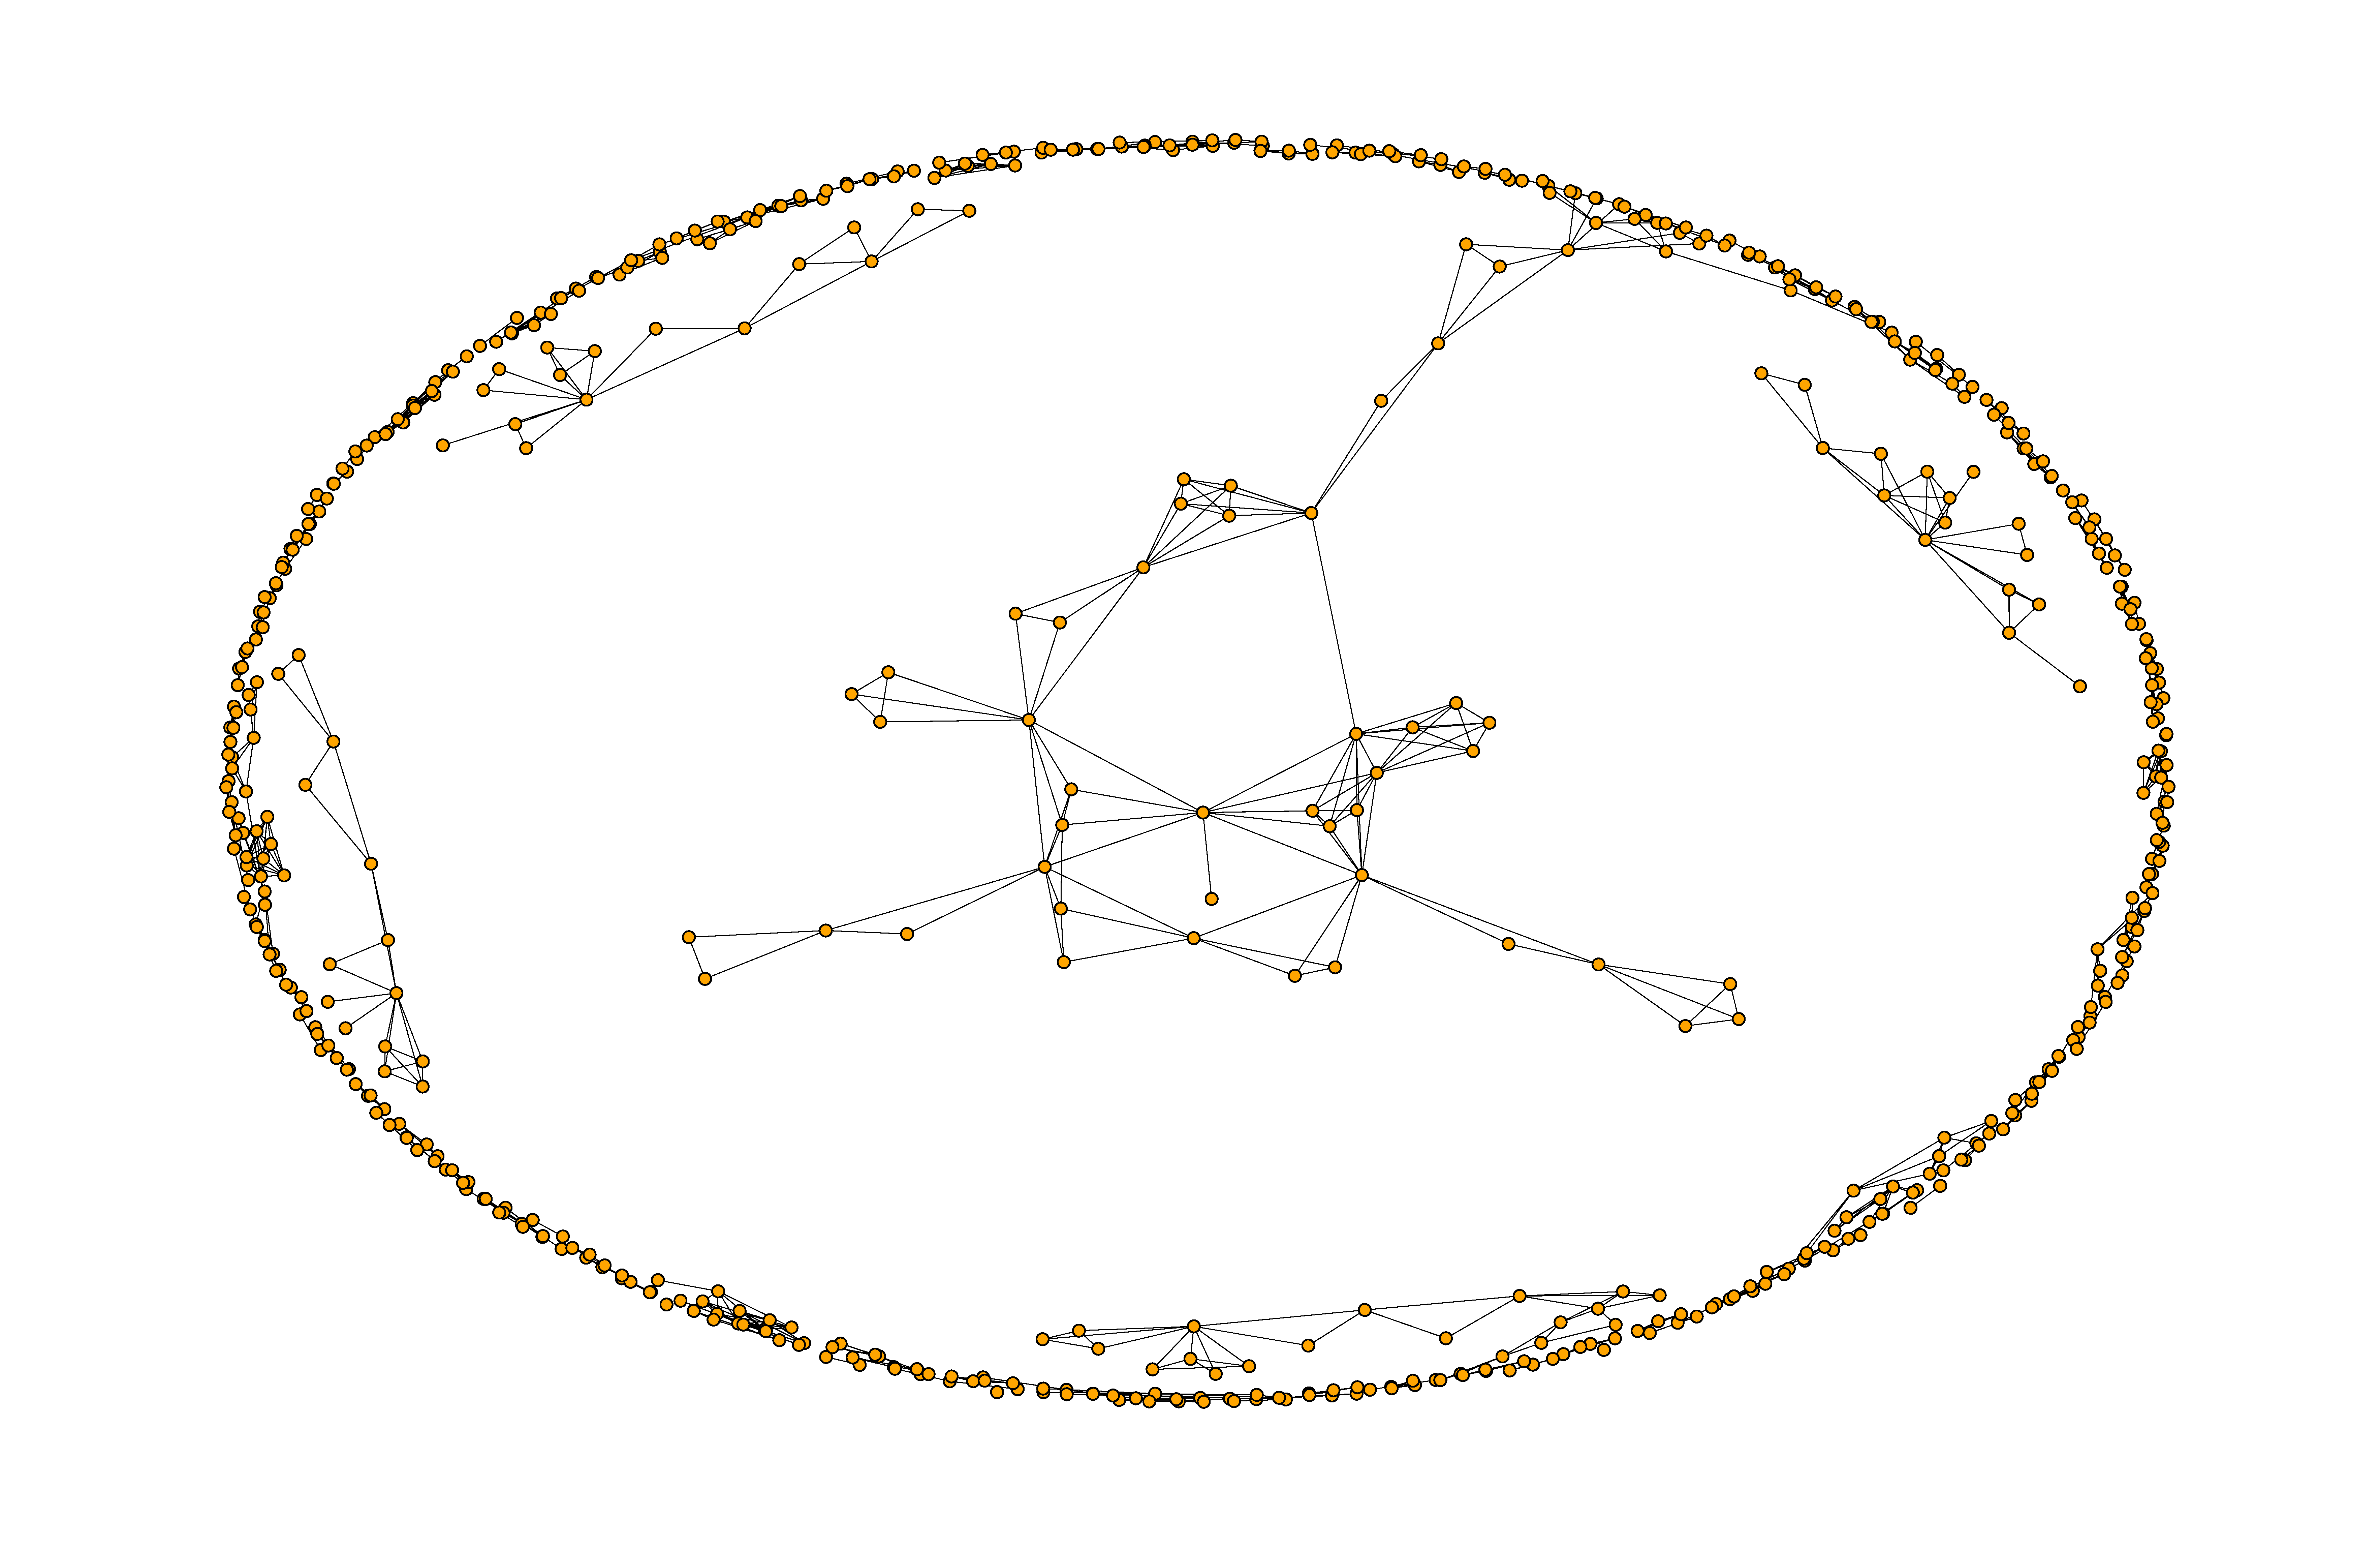
\includegraphics[width=\textwidth]{./assets/images/co-authors-network-price.pdf}
            \caption{Co authorship network for the price of anarchy.}
        \end{subfigure}
    \caption{Co authorship network for other topics.}
    \label{fig:co-authorship-other-topics}
    \end{figure}
    \end{center}

\subsubsection{Collaborative behaviour}

In this section we ascertain the level of collaborative nature of the field
using several connectivity measures. Several sub graphs of \(G\) will be used
as examples to explain the notion of some of these measures.

\paragraph{The measures}
\mbox{ }\\

The first measure introduced is the number of connected components.
A connected component of an undirected graph is a maximal set of nodes such that
each pair of nodes is connected by a path. Let us consider two graphs \(Z\) and
\(H\) (shown in Figure~\ref{fig:connected_components}), where \(V(Z), V(H)
\subseteq V (G)\) and \( E(Z), E(H) \subseteq E(G)\).

\begin{center}
\begin{figure}[!hbtp]
    \begin{subfigure}{0.5\textwidth}
        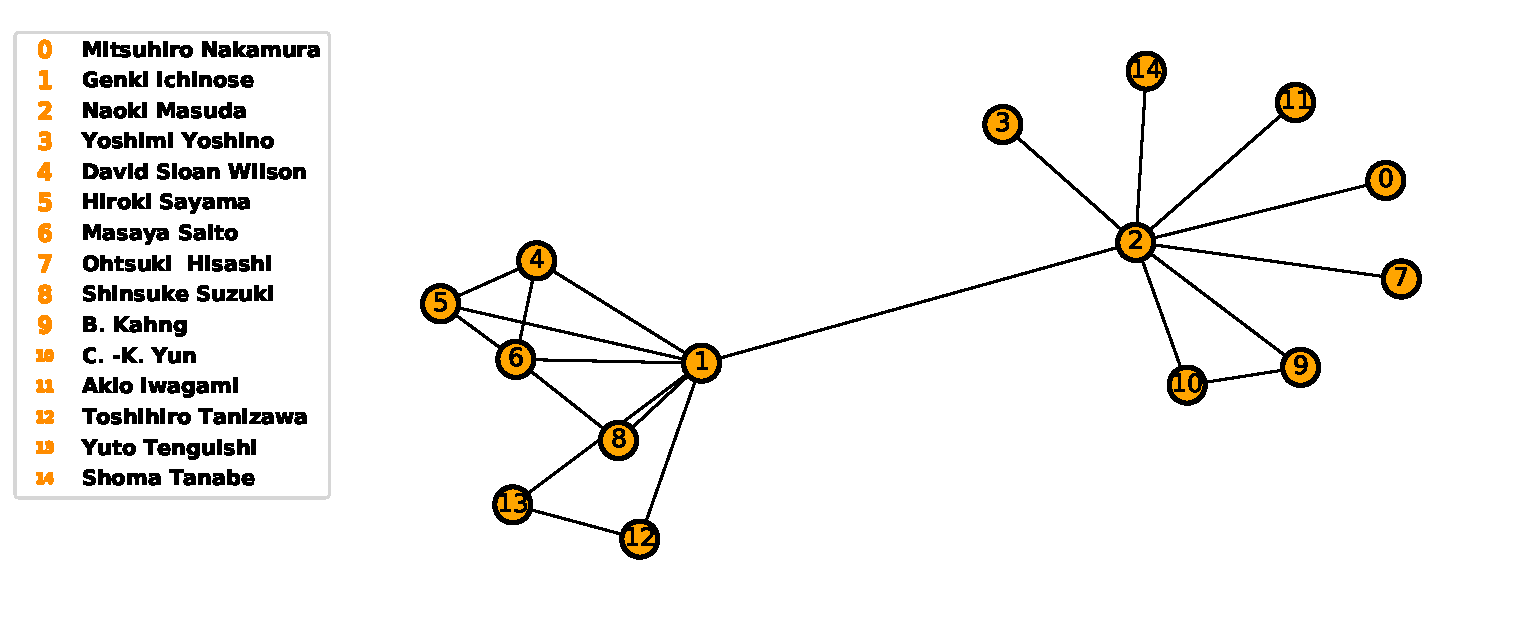
\includegraphics[width=\textwidth]{./assets/images/connected_example_one.pdf}
        \caption{A sub graph of \(G_1\) with 1 connected component.}
    \end{subfigure}
    \begin{subfigure}{0.5\textwidth}
        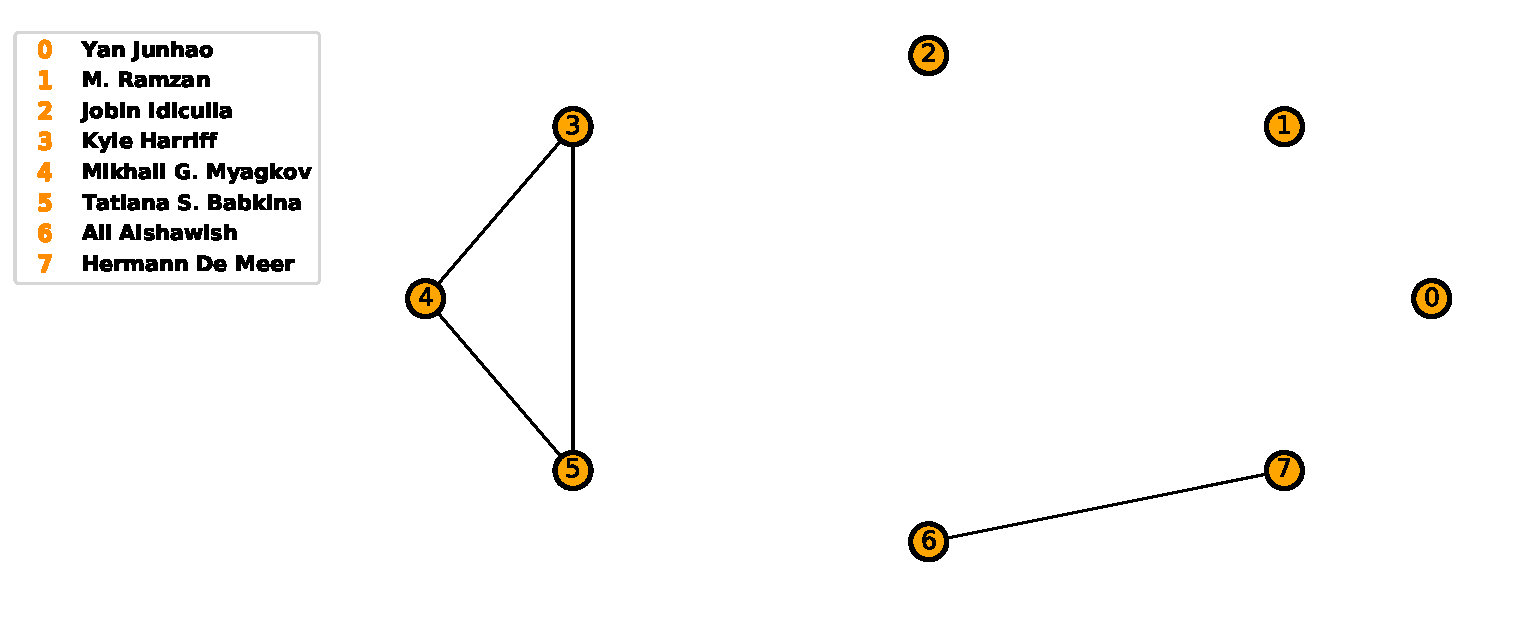
\includegraphics[width=\textwidth]{./assets/images/connected_example_two.pdf}
        \caption{A sub graph of \(G_1\) with 5 connected component.}
    \end{subfigure}
\caption{Connected components examples.}
\label{fig:connected_components}
\end{figure}
\end{center}

The number of connected components for sub graph \(Z\) is 1. On the other
hand the number of connected components for sub graph \(H\) is 5. Note that single
vertices are considered a connected component because they are connected by a path
to themselves. Due the nature of our study we are interested only in connected components
with more than one vertex, thus authors that have written with at least another
person. For the number of connected components we isolate the single vertices
and we count only those with at least two vertices.

The second connectivity measure considered is the clustering coefficient. Clustering
coefficient is a measure of the degree to which nodes in a graph tend to
cluster together, thus a measure of cliqueness. There are two version of this
meaurer, the local and the global. The local coefficient measures the clustering
coefficient of a single node and is calculated as,

\[C_i = \frac{2 \times N_E}{(I_degree)}\]

Number of edges between neighbours, Node degree (Node degree - 1).

The global coefficient is calculated by averaging all the local coefficients of
the graph. The values of the measure can range between \(0\) and \(1\). 

A clustering coefficient of \(1\) indicicates that the graph is a complete graph.
This case is not ideal in a co authorship network. Such a high coefficient would
indicate that teams of authors only write with each other, and not a sinle person
tends to collaborate with an external author (sub graph \(K\)). On the contrary,
a coefficient of \(0\) indicates
that authors write only with just a single co author, sub graph \(A\).
The case that lines in between is that of sub graph \(M\) where the clustering
coefficient has been estimated to be \(0.23\).

\begin{center}
    \begin{figure}[!hbtp]
        \begin{subfigure}{0.33\textwidth}
            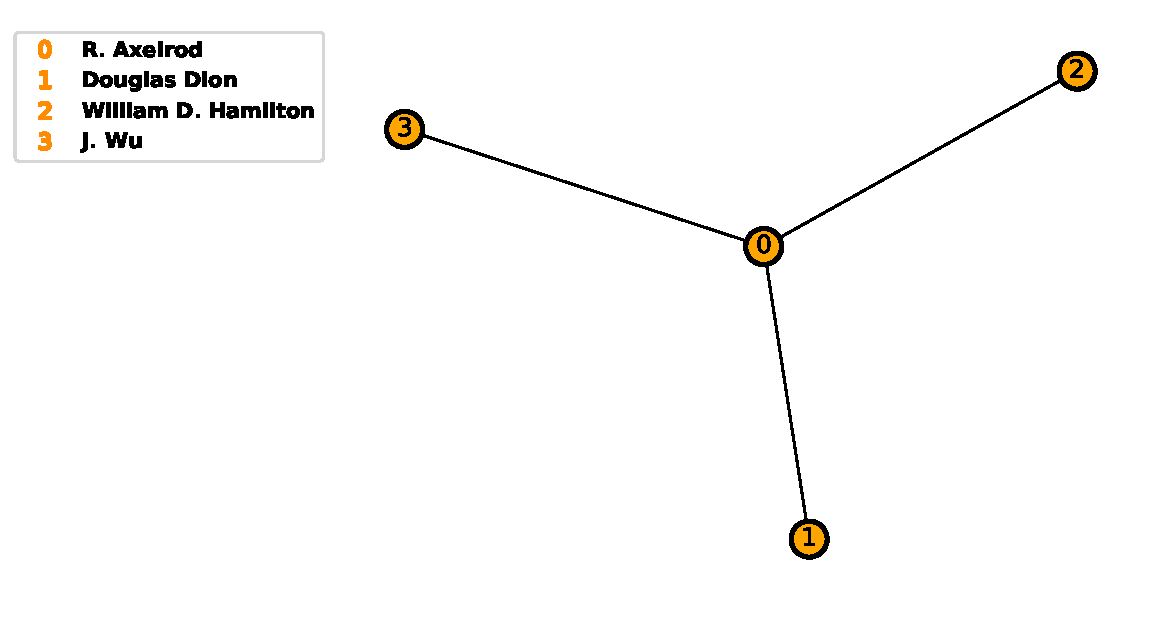
\includegraphics[width=\textwidth]{./assets/images/clustering_example_one.pdf}
            \caption{A sub graph of \(G_1\) with a clustering coefficient of 0.}
        \end{subfigure}
        \begin{subfigure}{0.33\textwidth}
            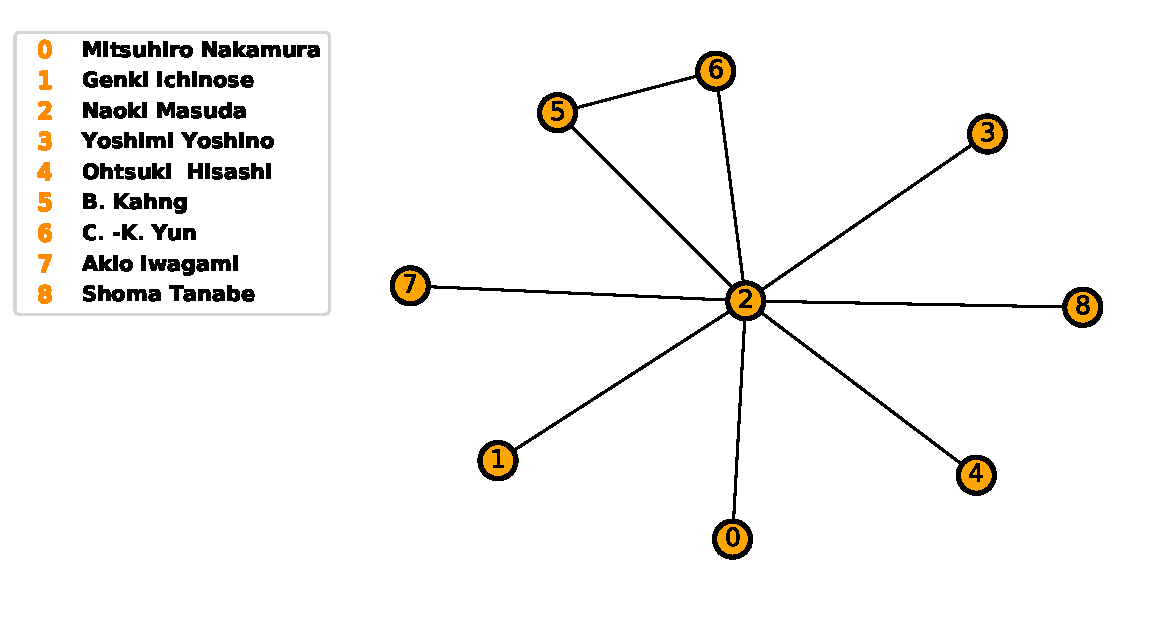
\includegraphics[width=\textwidth]{./assets/images/clustering_example_two.pdf}
            \caption{A sub graph of \(G_1\) with a clustering coefficient of 0.23.}
        \end{subfigure}
        \begin{subfigure}{0.33\textwidth}
            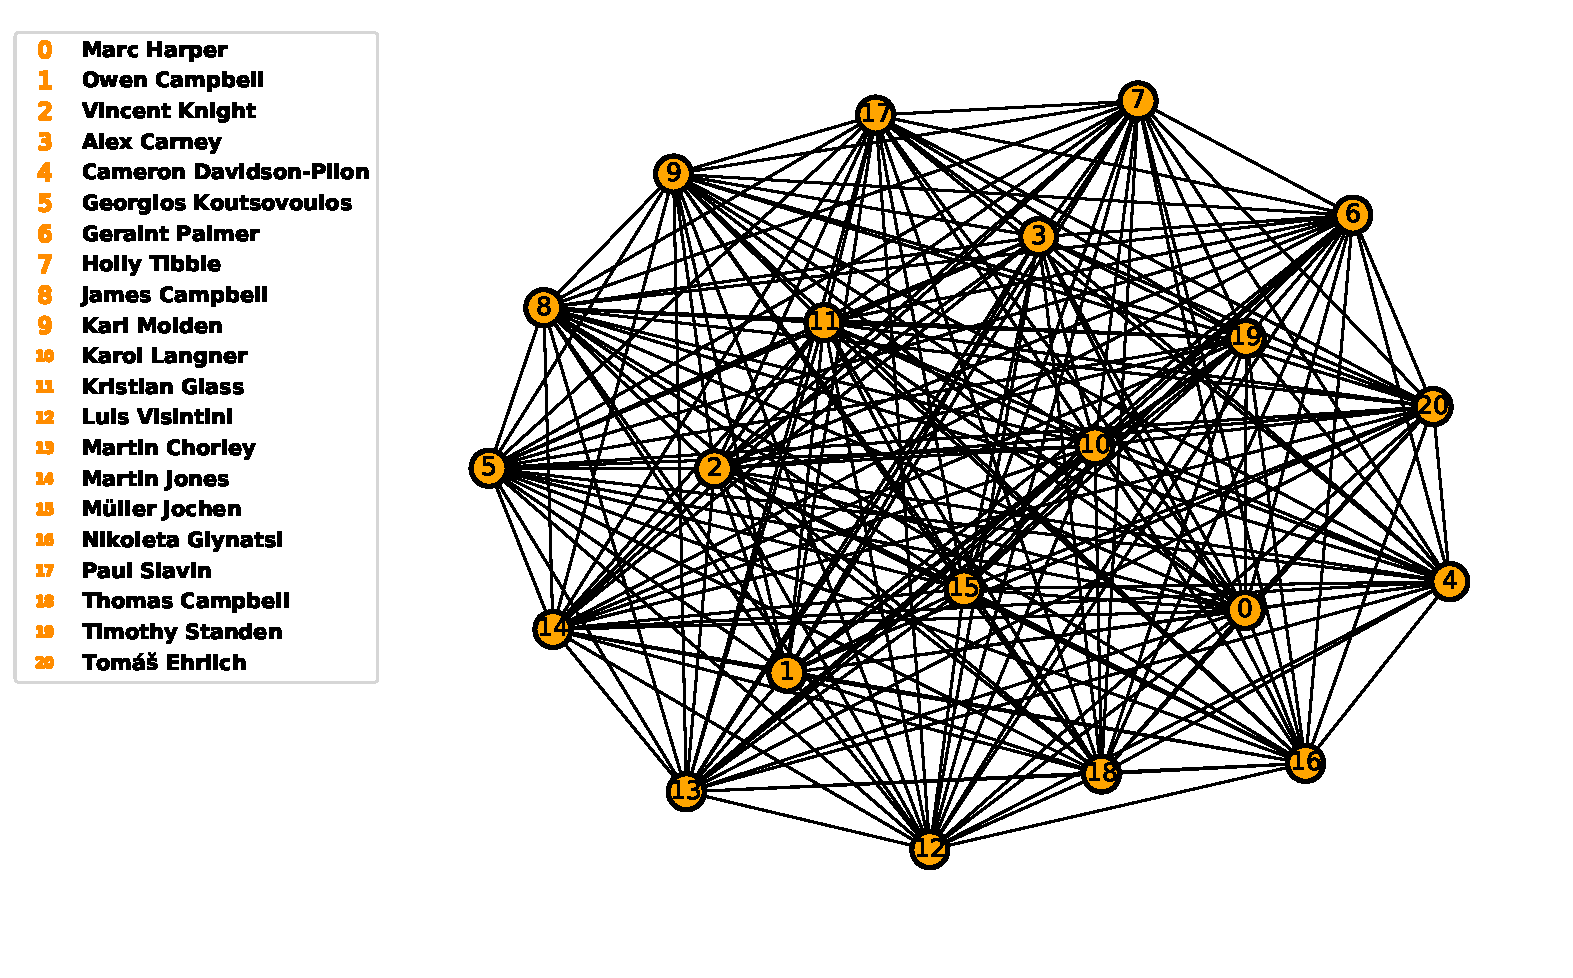
\includegraphics[width=\textwidth]{./assets/images/clustering_example_three.pdf}
            \caption{A sub graph of \(G_1\) with a clustering coefficient of 1.}
        \end{subfigure}
    \caption{Clustering coefficients examples.}
    \label{fig:clustering_coefficients}
    \end{figure}
    \end{center}

The final measure considered in this section is the degree distribution. Degree
shows the number of connections a node has. The degree distribution will allow
us to understand the most common degree in our networks.

\paragraph{Comparison with other topics co authorship}
\mbox{ }\\

All the above measure have been calculated for graph \(G\). Though we can not describe
how collaborative the network is without any comparison. Table~\ref{table:other_topics_cc}
summarises the measures for \(G\) and two other topics.

\begin{table}[!hbtp]
    \begin{center}
    \begin{tabular}{lcc}
        \toprule
                             & \textbf{Connected components} & \textbf{Clustering coefficient}\\
        \midrule
        Prisoner's dilemma   &                 \prisonerscon & \prisonerscc \\
        Auction games        &                   \auctioncon & \auctioncc   \\
        The price of anarchy &                     \pricecon & \pricecc     \\
        \bottomrule
    \end{tabular}
    \end{center}
    \caption{Collaborative behaviour measures for auction games and the price of anarchy.}
    \label{table:other_topics_cc}
\end{table}

Graphs \(G\) has a smaller number of connected components compared to the equivalent
graph for auction games. Even so, the global clustering coefficient of the two
networks is the same. This implies that authors of network \(G\) tend to collaborate
with more people. However, the field appears to be less collaborative compared
to the topic of price of anarchy, which has a clustering coefficient of 0.77 with
only 162 connected components.

To further examined the differences or the similarities of these networks we
consider the degree distributions. The normalised distributions of all
three networks are given in Figure~\ref{fig:degrees_dist}. They have been normalised
such that the frequencies sum to one. The distributions appear to be similar
but to validate the hypothesis a statistical test is used.

None of the distributions is normally distributed thus the non parametric test
Kruskal-Wallis is used~\cite{mckight2010}. Kruskal-Wallis allow us to compare the
medians of two or more distributions. The test returns a \(p\)-value of 0.29.
Thus, there is no significant difference in the degree distributions of the
three networks.

\begin{figure}[!hbtp]
    \centering
    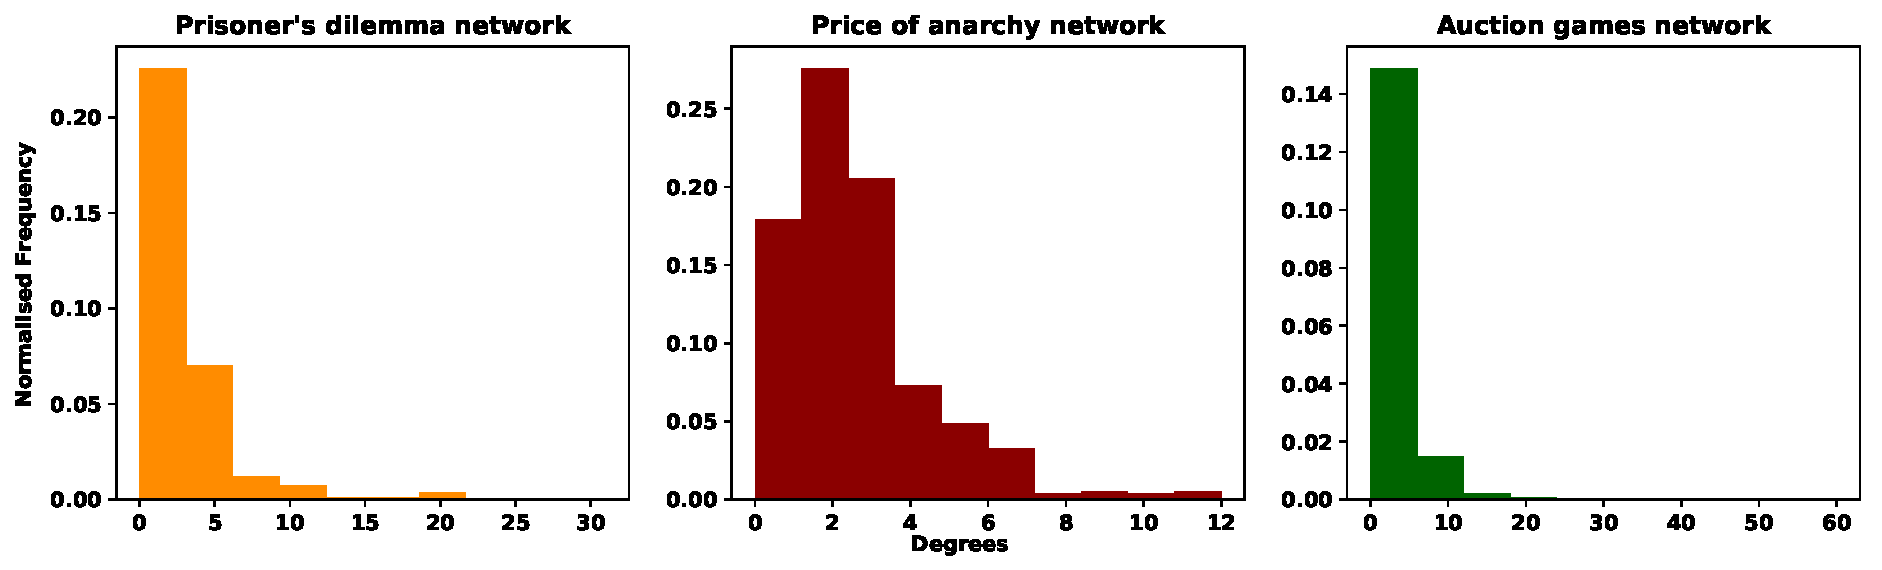
\includegraphics[width=\textwidth]{./assets/images/degrees_histrograms.pdf}
    \caption{Degree distributions for all three networks.}\label{fig:degrees_dist}
\end{figure}

\paragraph{Temporal comparison}
\mbox{ }\\

The collaborative behaviour of \(G\) is also studied over time. That is achieve
by calculating the number of connected components, the clustering coefficients and
the degrees distribution for each time period. Table~\ref{table:cc_over_time}
summarises the results.

Period 2 appears to be a very poor period of publication in our sources. There is
a single connected components, with an average clustering coefficient of 0. This
indicates collaboration with a single author.
Period 5 has the highest number of connected components but period 7 has the highest
clustering coefficient of 0.8 with only 108 connected components.
A big increase of connected components is spotted from periods 4 to 5.
Thus from period 2 onwards the field appears to be more collaborative, with most
collaborative period being the 7th.

Furthermore, over time the degree seems to be stabilising over 2 degrees, Figure
\ref{fig:dist_over_time}. Thus in the study of the prisoners dilemma according
to our data, papers with 3 authors seems to be favoured.

\begin{table}[!hbtp]
    \begin{center}
    \begin{tabular}{lcc}
        \toprule
                  & \textbf{Connected components} & \textbf{Clustering coefficient}\\
        \midrule
        period 1  & 12                            & 0.54 \\
        period 2  & 1                             & 0.0 \\
        period 3  & 14                            & 0.29 \\
        period 4  & 44                            & 0.44 \\
        period 5  & 411                           & 0.69 \\
        period 6  & 230                           & 0.78 \\
        period 7  & 108                           & 0.8 \\
        \bottomrule
    \end{tabular}
    \end{center}
    \caption{Collaborative behaviour measures over time periods.}
    \label{table:cc_over_time}
\end{table}

\begin{figure}[!hbtp]
    \centering
    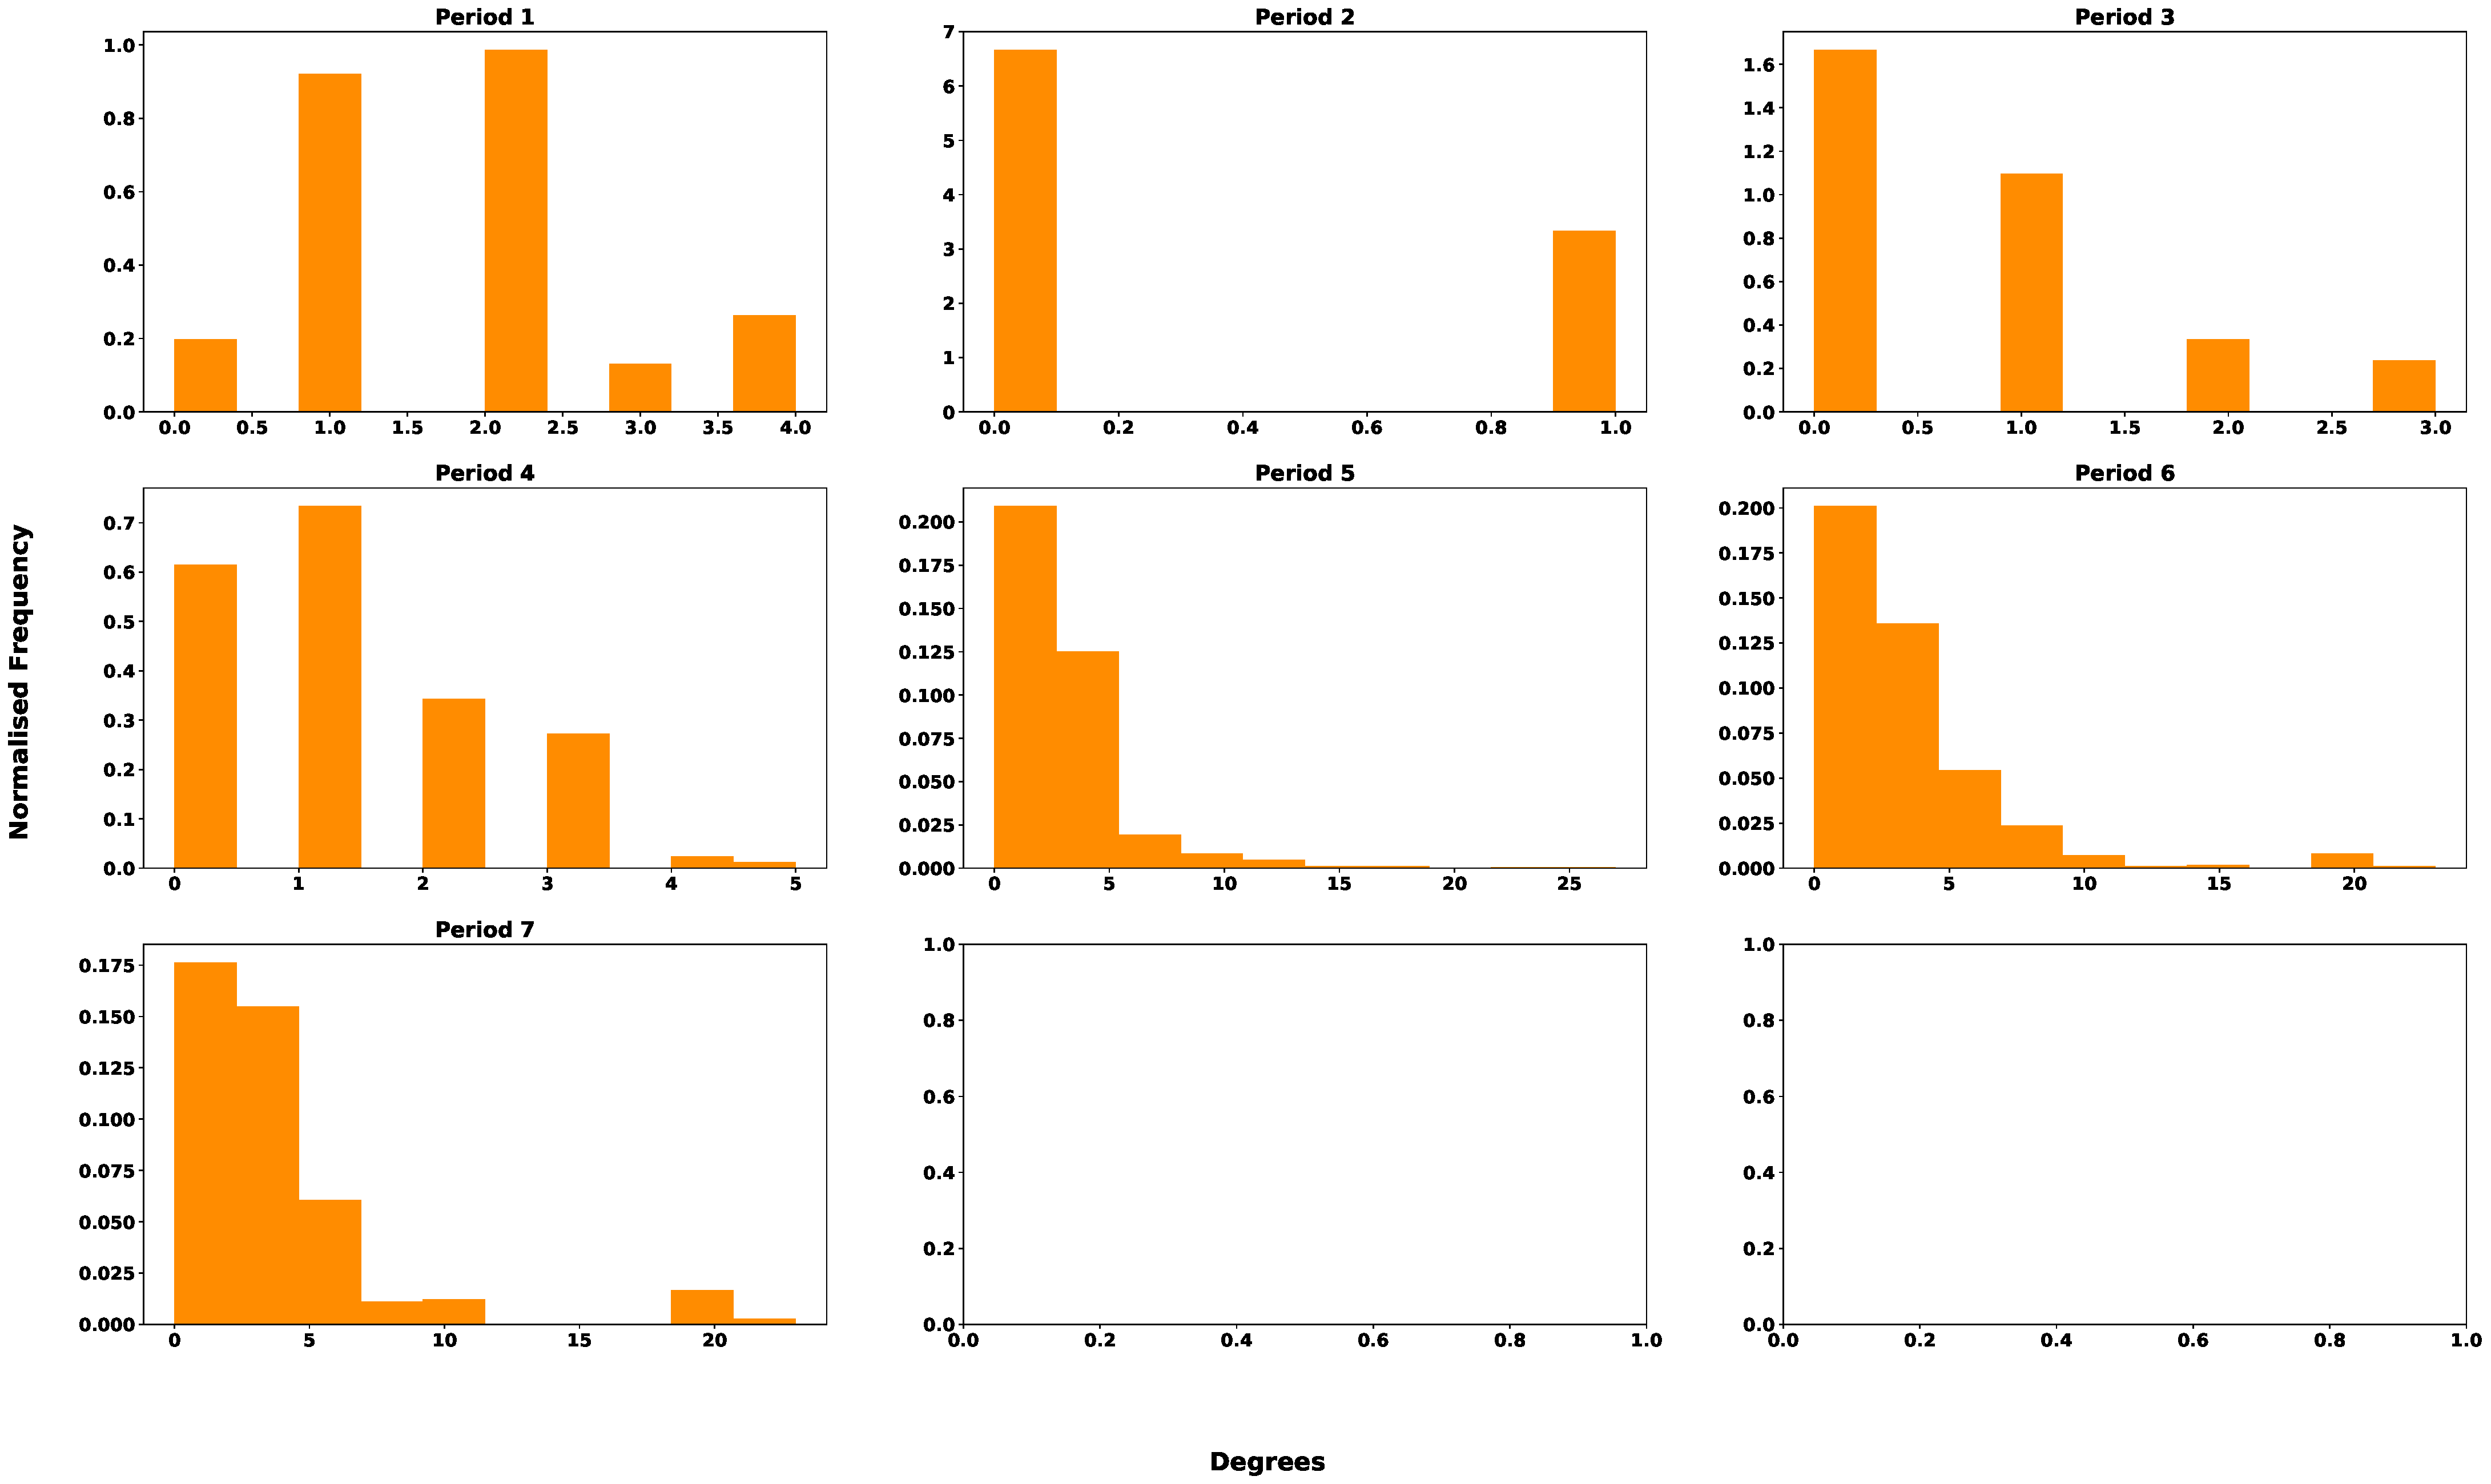
\includegraphics[width=0.8\textwidth]{./assets/images/degrees_histrograms_temporal.pdf}
    \caption{Degrees distribution over time.}\label{fig:dist_over_time}
\end{figure}

\subsubsection{Influence}

Network centrality is used in network theory to study which nodes of a graph are
the most important. There are several centrality measures used in different
projects to explain different behaviours of the nodes. Centrality will be used
here to explain influence. Two centrality measures are used here:

\begin{itemize}
    \item closeness centrality and
    \item betweenness centrality.
\end{itemize}

\paragraph{Measures}
\mbox{ }\\

Closeness centrality is used to explain which people influence the field and
betweenness centrality is used to explain which people gain from that influence.
Similarly both network measures are explained with an example.

\textbf{Closeness} centrality of a node \(u\) is the reciprocal of the average
shortest path distance to \(u\) over all \(n-1\) reachable nodes. It is denoted as,

\[C(u)= \frac{n - 1}{\displaystyle \Sigma_{v=1}^{n-1}d(v, u)}\]

where \(d(v, u)\) is the shortest-path distance between \(v\) and \(u\), and \(n\)
is the number of nodes that can reach \(u\). In our analysis we consider the
normalised closeness centrality which is normalised by the number of nodes in the
connected part of the graph.

\textbf{Betweenness} centrality of a node \(u\) is the sum of the fraction of all-pairs
shortest paths that pass through \(u\). It is denoted as,

\[ C_B(u)=\Sigma_{s,t \in V} \frac{\sigma (s,t|u)}{\sigma(s,t)}\]

where \(V\) is the set of nodes, \(\sigma(s,t)\) is the number of shortest \((s,t)\)-paths,
and \(\sigma(s,t|v)\) is the number of those paths passing through some node
\(u\) other than \(s,t\). If \(s=t\), \(\sigma(s,t)=1\), and if \(u \in s,t, \sigma(s,t|u)=0\).
Betweenness values are normalized by \(\frac{2}{((n-1)(n-2))}\).

Closeness is a measure that shows how well a node connects other nodes. Equivalently,
how well an author is connected to other authors and make them collaborate. 
This is called influence. On the other hand betweenness is about how connected a
node is, thus how much influence an author can gain from their environment.

As an example consider sub graph \(T\), Figure~\ref{fig:subgraph_t}. Note that
nodes 1, 2 and 3 are connected to three authors. Thus we expect their betweenness
centrality to be the same. However, this is not true for closeness centrality.
Node 3 is the connecting link between at least 4 people. Thus node 3
is the person in the sub graph that influences most authors. Node 3 also gains
influence due ot its rule in the team, but node 2 achieves the same without connecting
people as much as node 3.

\begin{figure}[!hbtp]
    \centering
    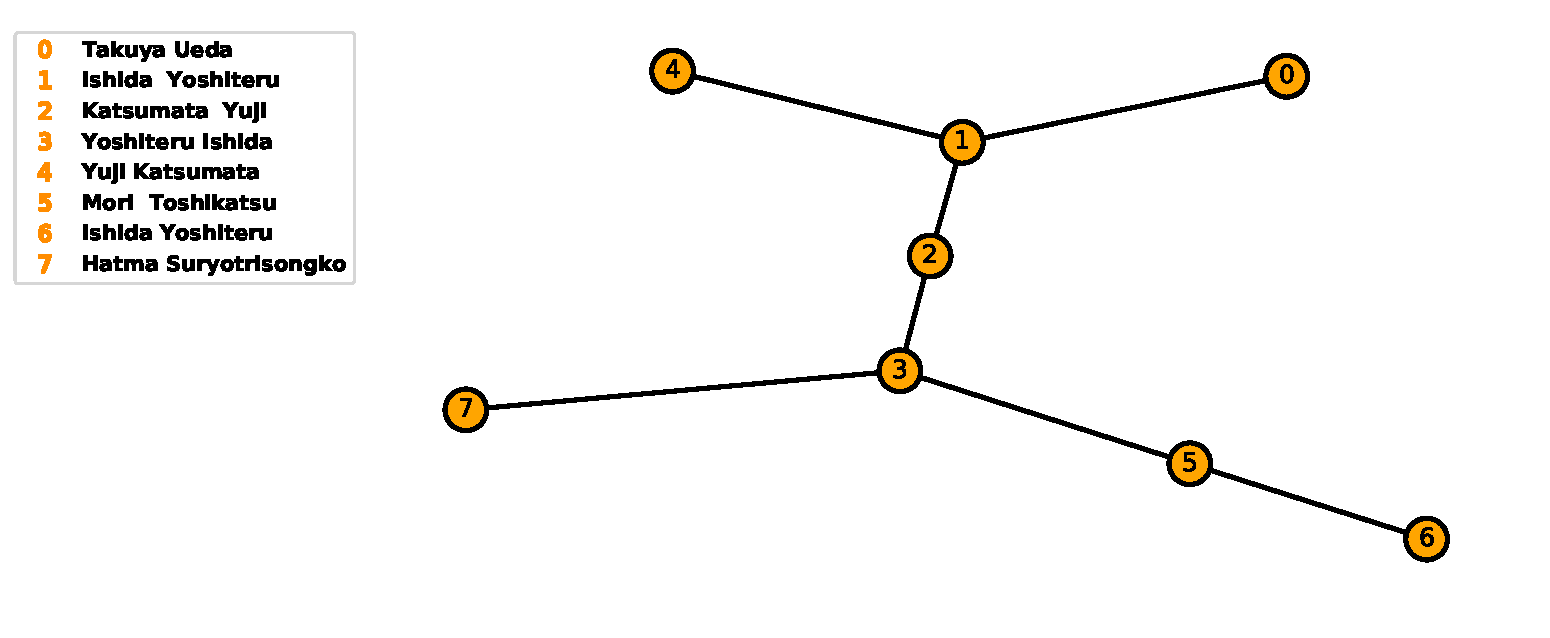
\includegraphics[width=0.8\textwidth]{./assets/images/centrality_example.pdf}
    \caption{A sub graph of \(G_1\).}\label{fig:subgraph_t}
\end{figure}

We identify those two measure to be important and we base our further analysis
on these measures. Due to an open source package called networkx the centrality
measures are easily calculated.
%ref networkx

Table~\ref{table:central_authors_pd} shows the most important authors of network
\(G\) based on the two centralities. The people that influence the field the most
are Matjaz Perc, Yamir Moreno, Luo-Luo Jiang, Arne Traulsen and Martin A. Nowak.
Their work have been discussed in Section~\ref{section:timeline}.
%Examples of their works.

Though Matjaz Perc and Yamir Moreno appear to both influence and gain from
the networks influence, it does not hold for the rest of the three authors.

\begin{table}[!hbtp]
    \begin{center}
    \scalebox{0.8}{
    \begin{tabular}{llr}
\toprule
{} &      Author name &  Betweeness \\
\midrule
1 &      Matjaz Perc &    0.010584 \\
2 &     Yamir Moreno &    0.008786 \\
3 &    Luo-Luo Jiang &    0.004319 \\
4 &    Arne Traulsen &    0.003920 \\
5 &  Martin A. Nowak &    0.003832 \\
\bottomrule
\end{tabular}

    \begin{tabular}{llr}
\toprule
{} &    Author name &  Closeness \\
\midrule
0 &    Matjaz Perc &   0.044428 \\
1 &   Yamir Moreno &   0.043561 \\
2 &   Cheng-Yi Xia &   0.038910 \\
3 &  Sandro Meloni &   0.037959 \\
4 &  Alberto Aleta &   0.037600 \\
\bottomrule
\end{tabular}
}
    \caption{Top 5 ranked authors based on different centrality measures.}
    \label{table:central_authors_pd}
    \end{center}
\end{table}

\paragraph{Comparison with other topics co authorship}
\mbox{ }\\

In order to compare the influence of the authors of different topics we
conduct pairwise comparisons of the centrality distributions of \(G\)
against the other topics. A total of \((2 \times 2)\) 4 statistical tests
are performed. Note that all distributions are not normally distributed thus a
non parametric test will be used. More specifically, the Mann-Whitney U 
test~\cite{nachar2008mann}.

Initially we test whether the median of the closeness centrality distribution
of \(G\) is equal or greater than the equivilent median of auction games.
Mann-Whitney U returns a \(p-\) value of 0. A similar test is conducted for
the betweenness centrality. This time we test that the median of \(G\) distribution
is equal or less. The results of our statical tests indicate that the prisoner's
dilemma authors tend to influence their field more than auction games authors.
However, the authors do not seem to gain as much from this influence.

The rest two Mann-Whitney U tests test whether the medians of the centralities
distribution of \(G\) are the same or less than the the equivilent medians for
the price of anarchy. Based on the \(p-\)values, the authors on the topic of price of
anarchy have both a stronger influence and gain from their co authorship connections
more than the authors of \(G\).

\paragraph{Temporal comparison}
\mbox{ }\\

The two centralities are also studied over time. Table~\ref{table:cc_over_time} higlights
the authors with the most influnce at each time period. Equivalently, Table~\ref{table:bc_over_time}
highlights the authors that gained more from the networks' influence at each
time period.

For periods 1, 3, 4, 5 and 6 the authors with the highest closeness centrality
are the authors with the highest betweenness centrality as well. Several of these
authors have been shown to also have a strong influence to the entire network
as well.

For period 7 though March Harper is the person that influences most authors,
Chen Yi Xia is the person that gains the most. For period 2 we have a similar
case. Robert Axelrod appears to be the most influenced author but not gaining 
as much from it.

Note that the centrality values are decreasing over the time periods. This could
be an effect due the size of the network which is increasing. Remember that
in smaller networks authors have more motivation to collaborate with the 
few people on their fields.

\begin{table}[!hbtp]
    \begin{center}
    \scalebox{0.8}{
    \begin{tabular}{llr}
\toprule
{} &      Author name &  Closeness \\
\midrule
1 &  Svenn Lindskold &   0.108108 \\
2 &       R. Axelrod &   0.200000 \\
3 &  Martin A. Nowak &   0.043478 \\
4 &  Lee A. Dugatkin &   0.029762 \\
5 &      Matjaz Perc &   0.043443 \\
6 &     Yamir Moreno &   0.039311 \\
7 &      Marc Harper &   0.049462 \\
\bottomrule
\end{tabular}
}
    \caption{Authors with the most influnce at each time period.}
    \label{table:cc_over_time}
    \end{center}
\end{table}

\begin{table}[!hbtp]
    \begin{center}
    \scalebox{0.8}{
    \begin{tabular}{llr}
\toprule
{} &      Author name &  Betweeness \\
\midrule
0 &  Svenn Lindskold &    0.006006 \\
1 &     A. W. Tucker &    0.000000 \\
2 &  Martin A. Nowak &    0.001279 \\
3 &  Lee A. Dugatkin &    0.000499 \\
4 &      Matjaz Perc &    0.010689 \\
5 &     Yamir Moreno &    0.005468 \\
6 &     Cheng-Yi Xia &    0.001242 \\
\bottomrule
\end{tabular}
}
    \caption{Authors that gained more from the networks influence at each
    time period.}
    \label{table:bc_over_time}
    \end{center}
\end{table}

\paragraph{Conclusion}
\mbox{ }\\

The conclusions for the collaborative behaviour of the field are discussed here.
The ranking based on the number of connected components for the three topics
is the following, auction games, the prisoner's dilemma and the price of anarchy.
Though this could be due the size of the data set of each respective topic.

The clustering coefficients allow us to conclude that that the prisoner's dilemma
is more collaborative, as field, compared to auction games but less than the 
price of anarchy. Note that the price of anarchy is a relative new topic. Thus
with less authors there is a higher change to collaborate with the few people
in your field.

The median degree was statistically proven to be the same over the three different
topics. Thus the above results hold for topics where the median connections
of an author is the same.

Based on the time periods the prisoner dilemma appears to have increased it's
collaborations since period 2. Note that period 2 is a poor period based on our
data. Period 5 to 7 re the most collaboratice of the field.
In this sub section we have studied the influncers and the people that gain
from the influence of their field. We have presented the authors within the
field of the prisoner's dilemma that fitted the descriptions.

Moreover, in order to compare the power of influnce of the field we conducted
statistical tests to compaire both measures of centrality against two other
topics of game theory. The results of the statistical tests have shown that,

\begin{itemize}
    \item The prisoner's dilemma authors have more influence than the authors of
    auction games.
    \item Though they appear to be gaining less from that influence compared to
    auction games.
    \item Finally, the price of anarchy has a stronger influence, both ways, than
    the prisoner's dilemma. 
\end{itemize}

Over time we have shown in the previous subsection that the field is becoming
more collaborative. Though due the number of possible connections and connected
components over the time, the power of influence is shown to be decreasing.


\newpage
\bibliographystyle{plain}
\bibliography{bibliography.bib}
\end{document}
